\documentclass[11pt]{article}

    \usepackage[breakable]{tcolorbox}
    \usepackage{parskip} % Stop auto-indenting (to mimic markdown behaviour)
    

    % Basic figure setup, for now with no caption control since it's done
    % automatically by Pandoc (which extracts ![](path) syntax from Markdown).
    \usepackage{graphicx}
    % Maintain compatibility with old templates. Remove in nbconvert 6.0
    \let\Oldincludegraphics\includegraphics
    % Ensure that by default, figures have no caption (until we provide a
    % proper Figure object with a Caption API and a way to capture that
    % in the conversion process - todo).
    \usepackage{caption}
    \DeclareCaptionFormat{nocaption}{}
    \captionsetup{format=nocaption,aboveskip=0pt,belowskip=0pt}

    \usepackage{float}
    \floatplacement{figure}{H} % forces figures to be placed at the correct location
    \usepackage{xcolor} % Allow colors to be defined
    \usepackage{enumerate} % Needed for markdown enumerations to work
    \usepackage{geometry} % Used to adjust the document margins
    \usepackage{amsmath} % Equations
    \usepackage{amssymb} % Equations
    \usepackage{textcomp} % defines textquotesingle
    % Hack from http://tex.stackexchange.com/a/47451/13684:
    \AtBeginDocument{%
        \def\PYZsq{\textquotesingle}% Upright quotes in Pygmentized code
    }
    \usepackage{upquote} % Upright quotes for verbatim code
    \usepackage{eurosym} % defines \euro

    \usepackage{iftex}
    \ifPDFTeX
        \usepackage[T1]{fontenc}
        \IfFileExists{alphabeta.sty}{
              \usepackage{alphabeta}
          }{
              \usepackage[mathletters]{ucs}
              \usepackage[utf8x]{inputenc}
          }
    \else
        \usepackage{fontspec}
        \usepackage{unicode-math}
    \fi

    \usepackage{fancyvrb} % verbatim replacement that allows latex
    \usepackage{grffile} % extends the file name processing of package graphics
                         % to support a larger range
    \makeatletter % fix for old versions of grffile with XeLaTeX
    \@ifpackagelater{grffile}{2019/11/01}
    {
      % Do nothing on new versions
    }
    {
      \def\Gread@@xetex#1{%
        \IfFileExists{"\Gin@base".bb}%
        {\Gread@eps{\Gin@base.bb}}%
        {\Gread@@xetex@aux#1}%
      }
    }
    \makeatother
    \usepackage[Export]{adjustbox} % Used to constrain images to a maximum size
    \adjustboxset{max size={0.9\linewidth}{0.9\paperheight}}

    % The hyperref package gives us a pdf with properly built
    % internal navigation ('pdf bookmarks' for the table of contents,
    % internal cross-reference links, web links for URLs, etc.)
    \usepackage{hyperref}
    % The default LaTeX title has an obnoxious amount of whitespace. By default,
    % titling removes some of it. It also provides customization options.
    \usepackage{titling}
    \usepackage{longtable} % longtable support required by pandoc >1.10
    \usepackage{booktabs}  % table support for pandoc > 1.12.2
    \usepackage{array}     % table support for pandoc >= 2.11.3
    \usepackage{calc}      % table minipage width calculation for pandoc >= 2.11.1
    \usepackage[inline]{enumitem} % IRkernel/repr support (it uses the enumerate* environment)
    \usepackage[normalem]{ulem} % ulem is needed to support strikethroughs (\sout)
                                % normalem makes italics be italics, not underlines
    \usepackage{soul}      % strikethrough (\st) support for pandoc >= 3.0.0
    \usepackage{mathrsfs}
    

    
    % Colors for the hyperref package
    \definecolor{urlcolor}{rgb}{0,.145,.698}
    \definecolor{linkcolor}{rgb}{.71,0.21,0.01}
    \definecolor{citecolor}{rgb}{.12,.54,.11}

    % ANSI colors
    \definecolor{ansi-black}{HTML}{3E424D}
    \definecolor{ansi-black-intense}{HTML}{282C36}
    \definecolor{ansi-red}{HTML}{E75C58}
    \definecolor{ansi-red-intense}{HTML}{B22B31}
    \definecolor{ansi-green}{HTML}{00A250}
    \definecolor{ansi-green-intense}{HTML}{007427}
    \definecolor{ansi-yellow}{HTML}{DDB62B}
    \definecolor{ansi-yellow-intense}{HTML}{B27D12}
    \definecolor{ansi-blue}{HTML}{208FFB}
    \definecolor{ansi-blue-intense}{HTML}{0065CA}
    \definecolor{ansi-magenta}{HTML}{D160C4}
    \definecolor{ansi-magenta-intense}{HTML}{A03196}
    \definecolor{ansi-cyan}{HTML}{60C6C8}
    \definecolor{ansi-cyan-intense}{HTML}{258F8F}
    \definecolor{ansi-white}{HTML}{C5C1B4}
    \definecolor{ansi-white-intense}{HTML}{A1A6B2}
    \definecolor{ansi-default-inverse-fg}{HTML}{FFFFFF}
    \definecolor{ansi-default-inverse-bg}{HTML}{000000}

    % common color for the border for error outputs.
    \definecolor{outerrorbackground}{HTML}{FFDFDF}

    % commands and environments needed by pandoc snippets
    % extracted from the output of `pandoc -s`
    \providecommand{\tightlist}{%
      \setlength{\itemsep}{0pt}\setlength{\parskip}{0pt}}
    \DefineVerbatimEnvironment{Highlighting}{Verbatim}{commandchars=\\\{\}}
    % Add ',fontsize=\small' for more characters per line
    \newenvironment{Shaded}{}{}
    \newcommand{\KeywordTok}[1]{\textcolor[rgb]{0.00,0.44,0.13}{\textbf{{#1}}}}
    \newcommand{\DataTypeTok}[1]{\textcolor[rgb]{0.56,0.13,0.00}{{#1}}}
    \newcommand{\DecValTok}[1]{\textcolor[rgb]{0.25,0.63,0.44}{{#1}}}
    \newcommand{\BaseNTok}[1]{\textcolor[rgb]{0.25,0.63,0.44}{{#1}}}
    \newcommand{\FloatTok}[1]{\textcolor[rgb]{0.25,0.63,0.44}{{#1}}}
    \newcommand{\CharTok}[1]{\textcolor[rgb]{0.25,0.44,0.63}{{#1}}}
    \newcommand{\StringTok}[1]{\textcolor[rgb]{0.25,0.44,0.63}{{#1}}}
    \newcommand{\CommentTok}[1]{\textcolor[rgb]{0.38,0.63,0.69}{\textit{{#1}}}}
    \newcommand{\OtherTok}[1]{\textcolor[rgb]{0.00,0.44,0.13}{{#1}}}
    \newcommand{\AlertTok}[1]{\textcolor[rgb]{1.00,0.00,0.00}{\textbf{{#1}}}}
    \newcommand{\FunctionTok}[1]{\textcolor[rgb]{0.02,0.16,0.49}{{#1}}}
    \newcommand{\RegionMarkerTok}[1]{{#1}}
    \newcommand{\ErrorTok}[1]{\textcolor[rgb]{1.00,0.00,0.00}{\textbf{{#1}}}}
    \newcommand{\NormalTok}[1]{{#1}}

    % Additional commands for more recent versions of Pandoc
    \newcommand{\ConstantTok}[1]{\textcolor[rgb]{0.53,0.00,0.00}{{#1}}}
    \newcommand{\SpecialCharTok}[1]{\textcolor[rgb]{0.25,0.44,0.63}{{#1}}}
    \newcommand{\VerbatimStringTok}[1]{\textcolor[rgb]{0.25,0.44,0.63}{{#1}}}
    \newcommand{\SpecialStringTok}[1]{\textcolor[rgb]{0.73,0.40,0.53}{{#1}}}
    \newcommand{\ImportTok}[1]{{#1}}
    \newcommand{\DocumentationTok}[1]{\textcolor[rgb]{0.73,0.13,0.13}{\textit{{#1}}}}
    \newcommand{\AnnotationTok}[1]{\textcolor[rgb]{0.38,0.63,0.69}{\textbf{\textit{{#1}}}}}
    \newcommand{\CommentVarTok}[1]{\textcolor[rgb]{0.38,0.63,0.69}{\textbf{\textit{{#1}}}}}
    \newcommand{\VariableTok}[1]{\textcolor[rgb]{0.10,0.09,0.49}{{#1}}}
    \newcommand{\ControlFlowTok}[1]{\textcolor[rgb]{0.00,0.44,0.13}{\textbf{{#1}}}}
    \newcommand{\OperatorTok}[1]{\textcolor[rgb]{0.40,0.40,0.40}{{#1}}}
    \newcommand{\BuiltInTok}[1]{{#1}}
    \newcommand{\ExtensionTok}[1]{{#1}}
    \newcommand{\PreprocessorTok}[1]{\textcolor[rgb]{0.74,0.48,0.00}{{#1}}}
    \newcommand{\AttributeTok}[1]{\textcolor[rgb]{0.49,0.56,0.16}{{#1}}}
    \newcommand{\InformationTok}[1]{\textcolor[rgb]{0.38,0.63,0.69}{\textbf{\textit{{#1}}}}}
    \newcommand{\WarningTok}[1]{\textcolor[rgb]{0.38,0.63,0.69}{\textbf{\textit{{#1}}}}}


    % Define a nice break command that doesn't care if a line doesn't already
    % exist.
    \def\br{\hspace*{\fill} \\* }
    % Math Jax compatibility definitions
    \def\gt{>}
    \def\lt{<}
    \let\Oldtex\TeX
    \let\Oldlatex\LaTeX
    \renewcommand{\TeX}{\textrm{\Oldtex}}
    \renewcommand{\LaTeX}{\textrm{\Oldlatex}}
    % Document parameters
    % Document title
    \title{Module6-HW}
    
    
    
    
    
    
    
% Pygments definitions
\makeatletter
\def\PY@reset{\let\PY@it=\relax \let\PY@bf=\relax%
    \let\PY@ul=\relax \let\PY@tc=\relax%
    \let\PY@bc=\relax \let\PY@ff=\relax}
\def\PY@tok#1{\csname PY@tok@#1\endcsname}
\def\PY@toks#1+{\ifx\relax#1\empty\else%
    \PY@tok{#1}\expandafter\PY@toks\fi}
\def\PY@do#1{\PY@bc{\PY@tc{\PY@ul{%
    \PY@it{\PY@bf{\PY@ff{#1}}}}}}}
\def\PY#1#2{\PY@reset\PY@toks#1+\relax+\PY@do{#2}}

\@namedef{PY@tok@w}{\def\PY@tc##1{\textcolor[rgb]{0.73,0.73,0.73}{##1}}}
\@namedef{PY@tok@c}{\let\PY@it=\textit\def\PY@tc##1{\textcolor[rgb]{0.24,0.48,0.48}{##1}}}
\@namedef{PY@tok@cp}{\def\PY@tc##1{\textcolor[rgb]{0.61,0.40,0.00}{##1}}}
\@namedef{PY@tok@k}{\let\PY@bf=\textbf\def\PY@tc##1{\textcolor[rgb]{0.00,0.50,0.00}{##1}}}
\@namedef{PY@tok@kp}{\def\PY@tc##1{\textcolor[rgb]{0.00,0.50,0.00}{##1}}}
\@namedef{PY@tok@kt}{\def\PY@tc##1{\textcolor[rgb]{0.69,0.00,0.25}{##1}}}
\@namedef{PY@tok@o}{\def\PY@tc##1{\textcolor[rgb]{0.40,0.40,0.40}{##1}}}
\@namedef{PY@tok@ow}{\let\PY@bf=\textbf\def\PY@tc##1{\textcolor[rgb]{0.67,0.13,1.00}{##1}}}
\@namedef{PY@tok@nb}{\def\PY@tc##1{\textcolor[rgb]{0.00,0.50,0.00}{##1}}}
\@namedef{PY@tok@nf}{\def\PY@tc##1{\textcolor[rgb]{0.00,0.00,1.00}{##1}}}
\@namedef{PY@tok@nc}{\let\PY@bf=\textbf\def\PY@tc##1{\textcolor[rgb]{0.00,0.00,1.00}{##1}}}
\@namedef{PY@tok@nn}{\let\PY@bf=\textbf\def\PY@tc##1{\textcolor[rgb]{0.00,0.00,1.00}{##1}}}
\@namedef{PY@tok@ne}{\let\PY@bf=\textbf\def\PY@tc##1{\textcolor[rgb]{0.80,0.25,0.22}{##1}}}
\@namedef{PY@tok@nv}{\def\PY@tc##1{\textcolor[rgb]{0.10,0.09,0.49}{##1}}}
\@namedef{PY@tok@no}{\def\PY@tc##1{\textcolor[rgb]{0.53,0.00,0.00}{##1}}}
\@namedef{PY@tok@nl}{\def\PY@tc##1{\textcolor[rgb]{0.46,0.46,0.00}{##1}}}
\@namedef{PY@tok@ni}{\let\PY@bf=\textbf\def\PY@tc##1{\textcolor[rgb]{0.44,0.44,0.44}{##1}}}
\@namedef{PY@tok@na}{\def\PY@tc##1{\textcolor[rgb]{0.41,0.47,0.13}{##1}}}
\@namedef{PY@tok@nt}{\let\PY@bf=\textbf\def\PY@tc##1{\textcolor[rgb]{0.00,0.50,0.00}{##1}}}
\@namedef{PY@tok@nd}{\def\PY@tc##1{\textcolor[rgb]{0.67,0.13,1.00}{##1}}}
\@namedef{PY@tok@s}{\def\PY@tc##1{\textcolor[rgb]{0.73,0.13,0.13}{##1}}}
\@namedef{PY@tok@sd}{\let\PY@it=\textit\def\PY@tc##1{\textcolor[rgb]{0.73,0.13,0.13}{##1}}}
\@namedef{PY@tok@si}{\let\PY@bf=\textbf\def\PY@tc##1{\textcolor[rgb]{0.64,0.35,0.47}{##1}}}
\@namedef{PY@tok@se}{\let\PY@bf=\textbf\def\PY@tc##1{\textcolor[rgb]{0.67,0.36,0.12}{##1}}}
\@namedef{PY@tok@sr}{\def\PY@tc##1{\textcolor[rgb]{0.64,0.35,0.47}{##1}}}
\@namedef{PY@tok@ss}{\def\PY@tc##1{\textcolor[rgb]{0.10,0.09,0.49}{##1}}}
\@namedef{PY@tok@sx}{\def\PY@tc##1{\textcolor[rgb]{0.00,0.50,0.00}{##1}}}
\@namedef{PY@tok@m}{\def\PY@tc##1{\textcolor[rgb]{0.40,0.40,0.40}{##1}}}
\@namedef{PY@tok@gh}{\let\PY@bf=\textbf\def\PY@tc##1{\textcolor[rgb]{0.00,0.00,0.50}{##1}}}
\@namedef{PY@tok@gu}{\let\PY@bf=\textbf\def\PY@tc##1{\textcolor[rgb]{0.50,0.00,0.50}{##1}}}
\@namedef{PY@tok@gd}{\def\PY@tc##1{\textcolor[rgb]{0.63,0.00,0.00}{##1}}}
\@namedef{PY@tok@gi}{\def\PY@tc##1{\textcolor[rgb]{0.00,0.52,0.00}{##1}}}
\@namedef{PY@tok@gr}{\def\PY@tc##1{\textcolor[rgb]{0.89,0.00,0.00}{##1}}}
\@namedef{PY@tok@ge}{\let\PY@it=\textit}
\@namedef{PY@tok@gs}{\let\PY@bf=\textbf}
\@namedef{PY@tok@gp}{\let\PY@bf=\textbf\def\PY@tc##1{\textcolor[rgb]{0.00,0.00,0.50}{##1}}}
\@namedef{PY@tok@go}{\def\PY@tc##1{\textcolor[rgb]{0.44,0.44,0.44}{##1}}}
\@namedef{PY@tok@gt}{\def\PY@tc##1{\textcolor[rgb]{0.00,0.27,0.87}{##1}}}
\@namedef{PY@tok@err}{\def\PY@bc##1{{\setlength{\fboxsep}{\string -\fboxrule}\fcolorbox[rgb]{1.00,0.00,0.00}{1,1,1}{\strut ##1}}}}
\@namedef{PY@tok@kc}{\let\PY@bf=\textbf\def\PY@tc##1{\textcolor[rgb]{0.00,0.50,0.00}{##1}}}
\@namedef{PY@tok@kd}{\let\PY@bf=\textbf\def\PY@tc##1{\textcolor[rgb]{0.00,0.50,0.00}{##1}}}
\@namedef{PY@tok@kn}{\let\PY@bf=\textbf\def\PY@tc##1{\textcolor[rgb]{0.00,0.50,0.00}{##1}}}
\@namedef{PY@tok@kr}{\let\PY@bf=\textbf\def\PY@tc##1{\textcolor[rgb]{0.00,0.50,0.00}{##1}}}
\@namedef{PY@tok@bp}{\def\PY@tc##1{\textcolor[rgb]{0.00,0.50,0.00}{##1}}}
\@namedef{PY@tok@fm}{\def\PY@tc##1{\textcolor[rgb]{0.00,0.00,1.00}{##1}}}
\@namedef{PY@tok@vc}{\def\PY@tc##1{\textcolor[rgb]{0.10,0.09,0.49}{##1}}}
\@namedef{PY@tok@vg}{\def\PY@tc##1{\textcolor[rgb]{0.10,0.09,0.49}{##1}}}
\@namedef{PY@tok@vi}{\def\PY@tc##1{\textcolor[rgb]{0.10,0.09,0.49}{##1}}}
\@namedef{PY@tok@vm}{\def\PY@tc##1{\textcolor[rgb]{0.10,0.09,0.49}{##1}}}
\@namedef{PY@tok@sa}{\def\PY@tc##1{\textcolor[rgb]{0.73,0.13,0.13}{##1}}}
\@namedef{PY@tok@sb}{\def\PY@tc##1{\textcolor[rgb]{0.73,0.13,0.13}{##1}}}
\@namedef{PY@tok@sc}{\def\PY@tc##1{\textcolor[rgb]{0.73,0.13,0.13}{##1}}}
\@namedef{PY@tok@dl}{\def\PY@tc##1{\textcolor[rgb]{0.73,0.13,0.13}{##1}}}
\@namedef{PY@tok@s2}{\def\PY@tc##1{\textcolor[rgb]{0.73,0.13,0.13}{##1}}}
\@namedef{PY@tok@sh}{\def\PY@tc##1{\textcolor[rgb]{0.73,0.13,0.13}{##1}}}
\@namedef{PY@tok@s1}{\def\PY@tc##1{\textcolor[rgb]{0.73,0.13,0.13}{##1}}}
\@namedef{PY@tok@mb}{\def\PY@tc##1{\textcolor[rgb]{0.40,0.40,0.40}{##1}}}
\@namedef{PY@tok@mf}{\def\PY@tc##1{\textcolor[rgb]{0.40,0.40,0.40}{##1}}}
\@namedef{PY@tok@mh}{\def\PY@tc##1{\textcolor[rgb]{0.40,0.40,0.40}{##1}}}
\@namedef{PY@tok@mi}{\def\PY@tc##1{\textcolor[rgb]{0.40,0.40,0.40}{##1}}}
\@namedef{PY@tok@il}{\def\PY@tc##1{\textcolor[rgb]{0.40,0.40,0.40}{##1}}}
\@namedef{PY@tok@mo}{\def\PY@tc##1{\textcolor[rgb]{0.40,0.40,0.40}{##1}}}
\@namedef{PY@tok@ch}{\let\PY@it=\textit\def\PY@tc##1{\textcolor[rgb]{0.24,0.48,0.48}{##1}}}
\@namedef{PY@tok@cm}{\let\PY@it=\textit\def\PY@tc##1{\textcolor[rgb]{0.24,0.48,0.48}{##1}}}
\@namedef{PY@tok@cpf}{\let\PY@it=\textit\def\PY@tc##1{\textcolor[rgb]{0.24,0.48,0.48}{##1}}}
\@namedef{PY@tok@c1}{\let\PY@it=\textit\def\PY@tc##1{\textcolor[rgb]{0.24,0.48,0.48}{##1}}}
\@namedef{PY@tok@cs}{\let\PY@it=\textit\def\PY@tc##1{\textcolor[rgb]{0.24,0.48,0.48}{##1}}}

\def\PYZbs{\char`\\}
\def\PYZus{\char`\_}
\def\PYZob{\char`\{}
\def\PYZcb{\char`\}}
\def\PYZca{\char`\^}
\def\PYZam{\char`\&}
\def\PYZlt{\char`\<}
\def\PYZgt{\char`\>}
\def\PYZsh{\char`\#}
\def\PYZpc{\char`\%}
\def\PYZdl{\char`\$}
\def\PYZhy{\char`\-}
\def\PYZsq{\char`\'}
\def\PYZdq{\char`\"}
\def\PYZti{\char`\~}
% for compatibility with earlier versions
\def\PYZat{@}
\def\PYZlb{[}
\def\PYZrb{]}
\makeatother


    % For linebreaks inside Verbatim environment from package fancyvrb.
    \makeatletter
        \newbox\Wrappedcontinuationbox
        \newbox\Wrappedvisiblespacebox
        \newcommand*\Wrappedvisiblespace {\textcolor{red}{\textvisiblespace}}
        \newcommand*\Wrappedcontinuationsymbol {\textcolor{red}{\llap{\tiny$\m@th\hookrightarrow$}}}
        \newcommand*\Wrappedcontinuationindent {3ex }
        \newcommand*\Wrappedafterbreak {\kern\Wrappedcontinuationindent\copy\Wrappedcontinuationbox}
        % Take advantage of the already applied Pygments mark-up to insert
        % potential linebreaks for TeX processing.
        %        {, <, #, %, $, ' and ": go to next line.
        %        _, }, ^, &, >, - and ~: stay at end of broken line.
        % Use of \textquotesingle for straight quote.
        \newcommand*\Wrappedbreaksatspecials {%
            \def\PYGZus{\discretionary{\char`\_}{\Wrappedafterbreak}{\char`\_}}%
            \def\PYGZob{\discretionary{}{\Wrappedafterbreak\char`\{}{\char`\{}}%
            \def\PYGZcb{\discretionary{\char`\}}{\Wrappedafterbreak}{\char`\}}}%
            \def\PYGZca{\discretionary{\char`\^}{\Wrappedafterbreak}{\char`\^}}%
            \def\PYGZam{\discretionary{\char`\&}{\Wrappedafterbreak}{\char`\&}}%
            \def\PYGZlt{\discretionary{}{\Wrappedafterbreak\char`\<}{\char`\<}}%
            \def\PYGZgt{\discretionary{\char`\>}{\Wrappedafterbreak}{\char`\>}}%
            \def\PYGZsh{\discretionary{}{\Wrappedafterbreak\char`\#}{\char`\#}}%
            \def\PYGZpc{\discretionary{}{\Wrappedafterbreak\char`\%}{\char`\%}}%
            \def\PYGZdl{\discretionary{}{\Wrappedafterbreak\char`\$}{\char`\$}}%
            \def\PYGZhy{\discretionary{\char`\-}{\Wrappedafterbreak}{\char`\-}}%
            \def\PYGZsq{\discretionary{}{\Wrappedafterbreak\textquotesingle}{\textquotesingle}}%
            \def\PYGZdq{\discretionary{}{\Wrappedafterbreak\char`\"}{\char`\"}}%
            \def\PYGZti{\discretionary{\char`\~}{\Wrappedafterbreak}{\char`\~}}%
        }
        % Some characters . , ; ? ! / are not pygmentized.
        % This macro makes them "active" and they will insert potential linebreaks
        \newcommand*\Wrappedbreaksatpunct {%
            \lccode`\~`\.\lowercase{\def~}{\discretionary{\hbox{\char`\.}}{\Wrappedafterbreak}{\hbox{\char`\.}}}%
            \lccode`\~`\,\lowercase{\def~}{\discretionary{\hbox{\char`\,}}{\Wrappedafterbreak}{\hbox{\char`\,}}}%
            \lccode`\~`\;\lowercase{\def~}{\discretionary{\hbox{\char`\;}}{\Wrappedafterbreak}{\hbox{\char`\;}}}%
            \lccode`\~`\:\lowercase{\def~}{\discretionary{\hbox{\char`\:}}{\Wrappedafterbreak}{\hbox{\char`\:}}}%
            \lccode`\~`\?\lowercase{\def~}{\discretionary{\hbox{\char`\?}}{\Wrappedafterbreak}{\hbox{\char`\?}}}%
            \lccode`\~`\!\lowercase{\def~}{\discretionary{\hbox{\char`\!}}{\Wrappedafterbreak}{\hbox{\char`\!}}}%
            \lccode`\~`\/\lowercase{\def~}{\discretionary{\hbox{\char`\/}}{\Wrappedafterbreak}{\hbox{\char`\/}}}%
            \catcode`\.\active
            \catcode`\,\active
            \catcode`\;\active
            \catcode`\:\active
            \catcode`\?\active
            \catcode`\!\active
            \catcode`\/\active
            \lccode`\~`\~
        }
    \makeatother

    \let\OriginalVerbatim=\Verbatim
    \makeatletter
    \renewcommand{\Verbatim}[1][1]{%
        %\parskip\z@skip
        \sbox\Wrappedcontinuationbox {\Wrappedcontinuationsymbol}%
        \sbox\Wrappedvisiblespacebox {\FV@SetupFont\Wrappedvisiblespace}%
        \def\FancyVerbFormatLine ##1{\hsize\linewidth
            \vtop{\raggedright\hyphenpenalty\z@\exhyphenpenalty\z@
                \doublehyphendemerits\z@\finalhyphendemerits\z@
                \strut ##1\strut}%
        }%
        % If the linebreak is at a space, the latter will be displayed as visible
        % space at end of first line, and a continuation symbol starts next line.
        % Stretch/shrink are however usually zero for typewriter font.
        \def\FV@Space {%
            \nobreak\hskip\z@ plus\fontdimen3\font minus\fontdimen4\font
            \discretionary{\copy\Wrappedvisiblespacebox}{\Wrappedafterbreak}
            {\kern\fontdimen2\font}%
        }%

        % Allow breaks at special characters using \PYG... macros.
        \Wrappedbreaksatspecials
        % Breaks at punctuation characters . , ; ? ! and / need catcode=\active
        \OriginalVerbatim[#1,codes*=\Wrappedbreaksatpunct]%
    }
    \makeatother

    % Exact colors from NB
    \definecolor{incolor}{HTML}{303F9F}
    \definecolor{outcolor}{HTML}{D84315}
    \definecolor{cellborder}{HTML}{CFCFCF}
    \definecolor{cellbackground}{HTML}{F7F7F7}

    % prompt
    \makeatletter
    \newcommand{\boxspacing}{\kern\kvtcb@left@rule\kern\kvtcb@boxsep}
    \makeatother
    \newcommand{\prompt}[4]{
        {\ttfamily\llap{{\color{#2}[#3]:\hspace{3pt}#4}}\vspace{-\baselineskip}}
    }
    

    
    % Prevent overflowing lines due to hard-to-break entities
    \sloppy
    % Setup hyperref package
    \hypersetup{
      breaklinks=true,  % so long urls are correctly broken across lines
      colorlinks=true,
      urlcolor=urlcolor,
      linkcolor=linkcolor,
      citecolor=citecolor,
      }
    % Slightly bigger margins than the latex defaults
    
    \geometry{verbose,tmargin=1in,bmargin=1in,lmargin=1in,rmargin=1in}
    
    

\begin{document}
    
    \maketitle
    
    

    
    \textbf{Problem1-LeetcodeQ 94-Binary Tree Inorder Traversal-Easy}

Given the root of a binary tree, return the inorder traversal of its
nodes' values.

\begin{figure}
\centering
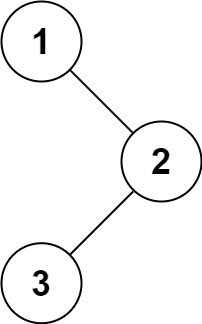
\includegraphics{ea7f99ce-c083-4a90-80d8-1f187e897165.jpg}
\caption{inorder\_1.jpg}
\end{figure}

\textbf{Example 1:}

\begin{itemize}
\tightlist
\item
  Input: root = {[}1,null,2,3{]}
\item
  Output: {[}1,3,2{]}
\end{itemize}

\textbf{Example 2:}

\begin{itemize}
\tightlist
\item
  Input: root = {[}{]}
\item
  Output: {[}{]}
\end{itemize}

\textbf{Example 3:}

\begin{itemize}
\tightlist
\item
  Input: root = {[}1{]}
\item
  Output: {[}1{]}
\end{itemize}

Constraints:

\begin{itemize}
\tightlist
\item
  The number of nodes in the tree is in the range {[}0, 100{]}.
\item
  -100 \textless= Node.val \textless= 100
\end{itemize}

    \subsubsection{Q94. Psuedocode}\label{q94.-psuedocode}

    \begin{tcolorbox}[breakable, size=fbox, boxrule=1pt, pad at break*=1mm,colback=cellbackground, colframe=cellborder]
\prompt{In}{incolor}{17}{\boxspacing}
\begin{Verbatim}[commandchars=\\\{\}]
\PY{n}{function} \PY{n}{inorder\PYZus{}traversal}\PY{p}{(}\PY{n}{root}\PY{p}{)}
\PY{n}{initialize} \PY{n}{empty} \PY{n+nb}{list} \PY{n}{res}
\PY{n}{initialize} \PY{n}{empty} \PY{n}{stack}
\PY{n+nb}{set} \PY{n}{p} \PY{n}{to} \PY{n}{root}
\PY{k}{while} \PY{n}{p} \PY{o+ow}{is} \PY{o+ow}{not} \PY{n}{null} \PY{o+ow}{or} \PY{n}{stack} \PY{o+ow}{is} \PY{o+ow}{not} \PY{n}{empty}
    \PY{k}{while} \PY{n}{p} \PY{o+ow}{is} \PY{o+ow}{not} \PY{n}{null}
        \PY{n}{push} \PY{n}{p} \PY{n}{to} \PY{n}{stack}
        \PY{n+nb}{set} \PY{n}{p} \PY{n}{to} \PY{n}{p}\PY{o}{.}\PY{n}{left}
    \PY{n+nb}{set} \PY{n}{p} \PY{n}{to} \PY{n}{stack}\PY{o}{.}\PY{n}{pop}\PY{p}{(}\PY{p}{)}
    \PY{n}{append} \PY{n}{p}\PY{o}{.}\PY{n}{val} \PY{n}{to} \PY{n}{res}
    \PY{n+nb}{set} \PY{n}{p} \PY{n}{to} \PY{n}{p}\PY{o}{.}\PY{n}{right}
\PY{k}{return} \PY{n}{res}
\end{Verbatim}
\end{tcolorbox}

    \begin{Verbatim}[commandchars=\\\{\}, frame=single, framerule=2mm, rulecolor=\color{outerrorbackground}]
\textcolor{ansi-cyan-intense}{\textbf{  Cell }}\textcolor{ansi-green-intense}{\textbf{In[17], line 1}}
\textcolor{ansi-yellow-intense}{\textbf{    function inorder\_traversal(root)}}
\textcolor{ansi-white-intense}{\textbf{             \^{}}}
\textcolor{ansi-red-intense}{\textbf{SyntaxError}}\textcolor{ansi-red-intense}{\textbf{:}} invalid syntax

    \end{Verbatim}

    \subsubsection{Q94. code.py}\label{q94.-code.py}

    \begin{tcolorbox}[breakable, size=fbox, boxrule=1pt, pad at break*=1mm,colback=cellbackground, colframe=cellborder]
\prompt{In}{incolor}{18}{\boxspacing}
\begin{Verbatim}[commandchars=\\\{\}]
\PY{k+kn}{from} \PY{n+nn}{typing} \PY{k+kn}{import} \PY{n}{List}\PY{p}{,} \PY{n}{Optional}
\PY{k}{class} \PY{n+nc}{TreeNode}\PY{p}{:}
    \PY{k}{def} \PY{n+nf+fm}{\PYZus{}\PYZus{}init\PYZus{}\PYZus{}}\PY{p}{(}\PY{n+nb+bp}{self}\PY{p}{,} \PY{n}{val}\PY{o}{=}\PY{l+m+mi}{0}\PY{p}{,} \PY{n}{left}\PY{o}{=}\PY{k+kc}{None}\PY{p}{,} \PY{n}{right}\PY{o}{=}\PY{k+kc}{None}\PY{p}{)}\PY{p}{:}
        \PY{n+nb+bp}{self}\PY{o}{.}\PY{n}{val} \PY{o}{=} \PY{n}{val}
        \PY{n+nb+bp}{self}\PY{o}{.}\PY{n}{left} \PY{o}{=} \PY{n}{left}
        \PY{n+nb+bp}{self}\PY{o}{.}\PY{n}{right} \PY{o}{=} \PY{n}{right}

\PY{k}{class} \PY{n+nc}{Solution}\PY{p}{:}
    \PY{k}{def} \PY{n+nf}{inorderTraversal}\PY{p}{(}\PY{n+nb+bp}{self}\PY{p}{,} \PY{n}{root}\PY{p}{:} \PY{n}{TreeNode}\PY{p}{)} \PY{o}{\PYZhy{}}\PY{o}{\PYZgt{}} \PY{n}{List}\PY{p}{[}\PY{n+nb}{int}\PY{p}{]}\PY{p}{:}
        \PY{n}{res} \PY{o}{=} \PY{p}{[}\PY{p}{]}
        \PY{n}{stack} \PY{o}{=} \PY{p}{[}\PY{p}{]}
        \PY{n}{p} \PY{o}{=} \PY{n}{root}
        \PY{k}{while} \PY{n}{p} \PY{o+ow}{or} \PY{n}{stack}\PY{p}{:}
            \PY{k}{while} \PY{n}{p}\PY{p}{:}
                \PY{n}{stack}\PY{o}{.}\PY{n}{append}\PY{p}{(}\PY{n}{p}\PY{p}{)}
                \PY{n}{p} \PY{o}{=} \PY{n}{p}\PY{o}{.}\PY{n}{left}
            \PY{n}{p} \PY{o}{=} \PY{n}{stack}\PY{o}{.}\PY{n}{pop}\PY{p}{(}\PY{p}{)}
            \PY{n}{res}\PY{o}{.}\PY{n}{append}\PY{p}{(}\PY{n}{p}\PY{o}{.}\PY{n}{val}\PY{p}{)}
            \PY{n}{p} \PY{o}{=} \PY{n}{p}\PY{o}{.}\PY{n}{right}
        \PY{k}{return} \PY{n}{res}

\PY{c+c1}{\PYZsh{} Creating the test case:}
\PY{n}{root} \PY{o}{=} \PY{n}{TreeNode}\PY{p}{(}\PY{l+m+mi}{1}\PY{p}{)}
\PY{n}{root}\PY{o}{.}\PY{n}{right} \PY{o}{=} \PY{n}{TreeNode}\PY{p}{(}\PY{l+m+mi}{2}\PY{p}{)}
\PY{n}{root}\PY{o}{.}\PY{n}{right}\PY{o}{.}\PY{n}{left} \PY{o}{=} \PY{n}{TreeNode}\PY{p}{(}\PY{l+m+mi}{3}\PY{p}{)}

\PY{c+c1}{\PYZsh{} Creating an instance of Solution and testing the method}
\PY{n}{solution} \PY{o}{=} \PY{n}{Solution}\PY{p}{(}\PY{p}{)}
\PY{n}{output} \PY{o}{=} \PY{n}{solution}\PY{o}{.}\PY{n}{inorderTraversal}\PY{p}{(}\PY{n}{root}\PY{p}{)}
\PY{n+nb}{print}\PY{p}{(}\PY{n}{output}\PY{p}{)}  \PY{c+c1}{\PYZsh{} Output should be [1, 3, 2]}
\end{Verbatim}
\end{tcolorbox}

    \begin{Verbatim}[commandchars=\\\{\}]
[1, 3, 2]
    \end{Verbatim}

    \textbf{Problem2-LeetcodeQ 230-Kth Smallest Element ina BST-Medium}

Given the root of a binary search tree, and an integer k, return the kth
smallest value (1-indexed) of all the values of the nodes in the tree.

\textbf{Example 1:}
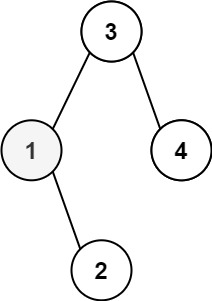
\includegraphics{7e8608b0-cb25-4352-ba0e-8f579aef1000.jpg}

\begin{itemize}
\tightlist
\item
  Input: root = {[}3,1,4,null,2{]}, k = 1
\item
  Output: 1
\end{itemize}

\textbf{Example 2:}
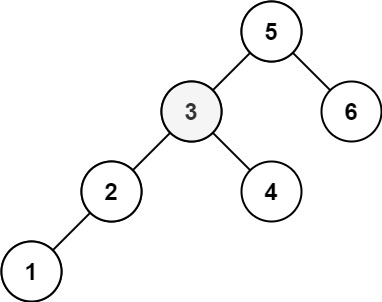
\includegraphics{41ccb892-f4bc-48f5-acbf-3896271d38a1.jpg}

\begin{itemize}
\tightlist
\item
  Input: root = {[}5,3,6,2,4,null,null,1{]}, k = 3
\item
  Output: 3
\end{itemize}

    \subsubsection{Q230. psuedocode}\label{q230.-psuedocode}

    \begin{tcolorbox}[breakable, size=fbox, boxrule=1pt, pad at break*=1mm,colback=cellbackground, colframe=cellborder]
\prompt{In}{incolor}{19}{\boxspacing}
\begin{Verbatim}[commandchars=\\\{\}]
\PY{n}{define} \PY{n}{inner} \PY{n}{function} \PY{n}{dfs}\PY{p}{(}\PY{n}{root}\PY{p}{)}
    \PY{k}{if} \PY{n}{root} \PY{o+ow}{is} \PY{n}{null}\PY{p}{,} \PY{k}{return}
    \PY{n}{call} \PY{n}{dfs}\PY{p}{(}\PY{n}{root}\PY{o}{.}\PY{n}{left}\PY{p}{)}
    \PY{k}{if} \PY{n}{k} \PY{o+ow}{is} \PY{n}{equal} \PY{n}{to} \PY{l+m+mi}{0}\PY{p}{,} \PY{k}{return}
    \PY{n}{decrement} \PY{n}{k} \PY{n}{by} \PY{l+m+mi}{1}
    \PY{k}{if} \PY{n}{k} \PY{o+ow}{is} \PY{n}{equal} \PY{n}{to} \PY{l+m+mi}{0}\PY{p}{,} \PY{n+nb}{set} \PY{n}{res} \PY{n}{to} \PY{n}{root}\PY{o}{.}\PY{n}{val}
    \PY{n}{call} \PY{n}{dfs}\PY{p}{(}\PY{n}{root}\PY{o}{.}\PY{n}{right}\PY{p}{)}
\PY{n+nb}{set} \PY{n}{k} \PY{n}{to} \PY{n+nb}{input} \PY{n}{k}
\PY{n}{call} \PY{n}{dfs}\PY{p}{(}\PY{n}{root}\PY{p}{)}
\PY{k}{return} \PY{n}{res}
\end{Verbatim}
\end{tcolorbox}

    \begin{Verbatim}[commandchars=\\\{\}, frame=single, framerule=2mm, rulecolor=\color{outerrorbackground}]
\textcolor{ansi-cyan-intense}{\textbf{  Cell }}\textcolor{ansi-green-intense}{\textbf{In[19], line 1}}
\textcolor{ansi-yellow-intense}{\textbf{    define inner function dfs(root)}}
\textcolor{ansi-white-intense}{\textbf{           \^{}}}
\textcolor{ansi-red-intense}{\textbf{SyntaxError}}\textcolor{ansi-red-intense}{\textbf{:}} invalid syntax

    \end{Verbatim}

    \subsubsection{Q230. code.py}\label{q230.-code.py}

    \begin{tcolorbox}[breakable, size=fbox, boxrule=1pt, pad at break*=1mm,colback=cellbackground, colframe=cellborder]
\prompt{In}{incolor}{8}{\boxspacing}
\begin{Verbatim}[commandchars=\\\{\}]
\PY{k+kn}{from} \PY{n+nn}{typing} \PY{k+kn}{import} \PY{n}{Optional}

\PY{k}{class} \PY{n+nc}{TreeNode}\PY{p}{:}
    \PY{k}{def} \PY{n+nf+fm}{\PYZus{}\PYZus{}init\PYZus{}\PYZus{}}\PY{p}{(}\PY{n+nb+bp}{self}\PY{p}{,} \PY{n}{val}\PY{o}{=}\PY{l+m+mi}{0}\PY{p}{,} \PY{n}{left}\PY{o}{=}\PY{k+kc}{None}\PY{p}{,} \PY{n}{right}\PY{o}{=}\PY{k+kc}{None}\PY{p}{)}\PY{p}{:}
        \PY{n+nb+bp}{self}\PY{o}{.}\PY{n}{val} \PY{o}{=} \PY{n}{val}
        \PY{n+nb+bp}{self}\PY{o}{.}\PY{n}{left} \PY{o}{=} \PY{n}{left}
        \PY{n+nb+bp}{self}\PY{o}{.}\PY{n}{right} \PY{o}{=} \PY{n}{right}

\PY{k}{class} \PY{n+nc}{Solution}\PY{p}{:}
    \PY{k}{def} \PY{n+nf}{kthSmallest}\PY{p}{(}\PY{n+nb+bp}{self}\PY{p}{,} \PY{n}{root}\PY{p}{:} \PY{n}{Optional}\PY{p}{[}\PY{n}{TreeNode}\PY{p}{]}\PY{p}{,} \PY{n}{k}\PY{p}{:} \PY{n+nb}{int}\PY{p}{)} \PY{o}{\PYZhy{}}\PY{o}{\PYZgt{}} \PY{n+nb}{int}\PY{p}{:}
        \PY{k}{def} \PY{n+nf}{dfs}\PY{p}{(}\PY{n}{root}\PY{p}{)}\PY{p}{:}
            \PY{k}{if} \PY{o+ow}{not} \PY{n}{root}\PY{p}{:}
                \PY{k}{return}
            \PY{n}{dfs}\PY{p}{(}\PY{n}{root}\PY{o}{.}\PY{n}{left}\PY{p}{)}
            \PY{k}{if} \PY{n+nb+bp}{self}\PY{o}{.}\PY{n}{k} \PY{o}{==} \PY{l+m+mi}{0}\PY{p}{:}
                \PY{k}{return}
            \PY{n+nb+bp}{self}\PY{o}{.}\PY{n}{k} \PY{o}{\PYZhy{}}\PY{o}{=} \PY{l+m+mi}{1}
            \PY{k}{if} \PY{n+nb+bp}{self}\PY{o}{.}\PY{n}{k} \PY{o}{==} \PY{l+m+mi}{0}\PY{p}{:}
                \PY{n+nb+bp}{self}\PY{o}{.}\PY{n}{res} \PY{o}{=} \PY{n}{root}\PY{o}{.}\PY{n}{val}
            \PY{n}{dfs}\PY{p}{(}\PY{n}{root}\PY{o}{.}\PY{n}{right}\PY{p}{)}

        \PY{n+nb+bp}{self}\PY{o}{.}\PY{n}{k} \PY{o}{=} \PY{n}{k}
        \PY{n}{dfs}\PY{p}{(}\PY{n}{root}\PY{p}{)}
        \PY{k}{return} \PY{n+nb+bp}{self}\PY{o}{.}\PY{n}{res}


\PY{n}{root} \PY{o}{=} \PY{n}{TreeNode}\PY{p}{(}\PY{l+m+mi}{3}\PY{p}{)}
\PY{n}{root}\PY{o}{.}\PY{n}{left} \PY{o}{=} \PY{n}{TreeNode}\PY{p}{(}\PY{l+m+mi}{1}\PY{p}{)}
\PY{n}{root}\PY{o}{.}\PY{n}{right} \PY{o}{=} \PY{n}{TreeNode}\PY{p}{(}\PY{l+m+mi}{4}\PY{p}{)}
\PY{n}{root}\PY{o}{.}\PY{n}{left}\PY{o}{.}\PY{n}{right} \PY{o}{=} \PY{n}{TreeNode}\PY{p}{(}\PY{l+m+mi}{2}\PY{p}{)}

\PY{c+c1}{\PYZsh{} Creating an instance of Solution and testing the method}
\PY{n}{solution} \PY{o}{=} \PY{n}{Solution}\PY{p}{(}\PY{p}{)}
\PY{n}{output} \PY{o}{=} \PY{n}{solution}\PY{o}{.}\PY{n}{kthSmallest}\PY{p}{(}\PY{n}{root}\PY{p}{,} \PY{l+m+mi}{1}\PY{p}{)}
\PY{n+nb}{print}\PY{p}{(}\PY{n}{output}\PY{p}{)} 
\end{Verbatim}
\end{tcolorbox}

    \begin{Verbatim}[commandchars=\\\{\}]
1
    \end{Verbatim}

    \textbf{Problem3-LeetcodeQ 105-Construct Binary Tree from Preorder and
Inorder Traversal-Medium}

Given two integer arrays preorder and inorder where preorder is the
preorder traversal of a binary tree and inorder is the inorder traversal
of the same tree, construct and return the binary tree.

\textbf{Example 1:}

\begin{figure}
\centering
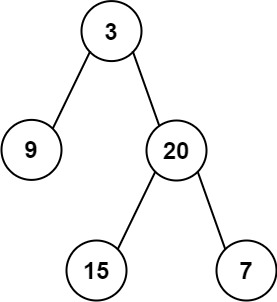
\includegraphics{0d9e8e38-5da2-4a3b-8a53-ee74e83c7ee5.jpg}
\caption{tree.jpg}
\end{figure}

\begin{itemize}
\tightlist
\item
  Input: preorder = {[}3,9,20,15,7{]}, inorder = {[}9,3,15,20,7{]}
\item
  Output: {[}3,9,20,null,null,15,7{]}
\end{itemize}

\textbf{Example 2:}

\begin{itemize}
\tightlist
\item
  Input: preorder = {[}-1{]}, inorder = {[}-1{]}
\item
  Output: {[}-1{]}
\end{itemize}

    \subsubsection{Q150. pseudocode}\label{q150.-pseudocode}

The algorithm works by leveraging the properties of preorder and inorder
tree traversals to reconstruct the binary tree.

In a preorder traversal, the first element is always the root of the
tree. The inorder traversal helps determine the structure of the tree by
providing the relative positions of the nodes with respect to the root.

The algorithm begins by identifying the root from the first element of
the preorder list. It then finds the root's position in the inorder
list, which divides the inorder list into left and right subtrees. The
left subtree consists of elements before the root in the inorder list,
and the right subtree consists of elements after the root. The algorithm
recursively applies the same logic to the left and right subtrees, using
appropriate slices of the preorder and inorder lists. This recursive
process continues until the entire tree is reconstructed.

The correctness is guaranteed because each recursive call precisely
identifies the root and splits the tree into left and right subtrees
based on the consistent properties of preorder and inorder traversals.

    \begin{tcolorbox}[breakable, size=fbox, boxrule=1pt, pad at break*=1mm,colback=cellbackground, colframe=cellborder]
\prompt{In}{incolor}{ }{\boxspacing}
\begin{Verbatim}[commandchars=\\\{\}]
\PY{n}{function} \PY{n}{build\PYZus{}tree}\PY{p}{(}\PY{n}{preorder}\PY{p}{,} \PY{n}{inorder}\PY{p}{)}
\PY{k}{if} \PY{n}{preorder} \PY{o+ow}{is} \PY{n}{empty}
    \PY{k}{return} \PY{n}{null}
\PY{n+nb}{set} \PY{n}{left\PYZus{}size} \PY{n}{to} \PY{n}{the} \PY{n}{index} \PY{n}{of} \PY{n}{preorder}\PY{p}{[}\PY{l+m+mi}{0}\PY{p}{]} \PY{o+ow}{in} \PY{n}{inorder}
\PY{n+nb}{set} \PY{n}{left} \PY{n}{to} \PY{n}{the} \PY{n}{result} \PY{n}{of} \PY{n}{calling} \PY{n}{build\PYZus{}tree} \PY{k}{with} 
    \PY{n}{preorder} \PY{k+kn}{from} \PY{n+nn}{index} \PY{l+m+mi}{1} \PY{n}{to} \PY{l+m+mi}{1} \PY{o}{+} \PY{n}{left\PYZus{}size} \PY{o+ow}{and} 
    \PY{n}{inorder} \PY{k+kn}{from} \PY{n+nn}{start} \PY{n}{to} \PY{n}{left\PYZus{}size}
\PY{n+nb}{set} \PY{n}{right} \PY{n}{to} \PY{n}{the} \PY{n}{result} \PY{n}{of} \PY{n}{calling} \PY{n}{build\PYZus{}tree} \PY{k}{with} 
    \PY{n}{preorder} \PY{k+kn}{from} \PY{l+m+mi}{1} \PY{o}{+} \PY{n}{left\PYZus{}size} \PY{n}{to} \PY{n}{end} \PY{o+ow}{and} 
    \PY{n}{inorder} \PY{k+kn}{from} \PY{l+m+mi}{1} \PY{o}{+} \PY{n}{left\PYZus{}size} \PY{n}{to} \PY{n}{end}
\PY{k}{return} \PY{n}{a} \PY{n}{new} \PY{n}{TreeNode} \PY{k}{with} \PY{n}{value} \PY{n}{preorder}\PY{p}{[}\PY{l+m+mi}{0}\PY{p}{]}\PY{p}{,} \PY{n}{left}\PY{p}{,} \PY{o+ow}{and} \PY{n}{right}
\end{Verbatim}
\end{tcolorbox}

    \subsubsection{Q150. code.py}\label{q150.-code.py}

    \begin{tcolorbox}[breakable, size=fbox, boxrule=1pt, pad at break*=1mm,colback=cellbackground, colframe=cellborder]
\prompt{In}{incolor}{11}{\boxspacing}
\begin{Verbatim}[commandchars=\\\{\}]
\PY{k+kn}{from} \PY{n+nn}{typing} \PY{k+kn}{import} \PY{n}{List}\PY{p}{,} \PY{n}{Optional}

\PY{k}{class} \PY{n+nc}{TreeNode}\PY{p}{:}
    \PY{k}{def} \PY{n+nf+fm}{\PYZus{}\PYZus{}init\PYZus{}\PYZus{}}\PY{p}{(}\PY{n+nb+bp}{self}\PY{p}{,} \PY{n}{val}\PY{o}{=}\PY{l+m+mi}{0}\PY{p}{,} \PY{n}{left}\PY{o}{=}\PY{k+kc}{None}\PY{p}{,} \PY{n}{right}\PY{o}{=}\PY{k+kc}{None}\PY{p}{)}\PY{p}{:}
        \PY{n+nb+bp}{self}\PY{o}{.}\PY{n}{val} \PY{o}{=} \PY{n}{val}
        \PY{n+nb+bp}{self}\PY{o}{.}\PY{n}{left} \PY{o}{=} \PY{n}{left}
        \PY{n+nb+bp}{self}\PY{o}{.}\PY{n}{right} \PY{o}{=} \PY{n}{right}

\PY{k}{class} \PY{n+nc}{Solution}\PY{p}{:}
    \PY{k}{def} \PY{n+nf}{buildTree}\PY{p}{(}\PY{n+nb+bp}{self}\PY{p}{,} \PY{n}{preorder}\PY{p}{:} \PY{n}{List}\PY{p}{[}\PY{n+nb}{int}\PY{p}{]}\PY{p}{,} \PY{n}{inorder}\PY{p}{:} \PY{n}{List}\PY{p}{[}\PY{n+nb}{int}\PY{p}{]}\PY{p}{)} \PY{o}{\PYZhy{}}\PY{o}{\PYZgt{}} \PY{n}{Optional}\PY{p}{[}\PY{n}{TreeNode}\PY{p}{]}\PY{p}{:}
        \PY{k}{if} \PY{o+ow}{not} \PY{n}{preorder}\PY{p}{:}
            \PY{k}{return} \PY{k+kc}{None}
        \PY{n}{left\PYZus{}size} \PY{o}{=} \PY{n}{inorder}\PY{o}{.}\PY{n}{index}\PY{p}{(}\PY{n}{preorder}\PY{p}{[}\PY{l+m+mi}{0}\PY{p}{]}\PY{p}{)}
        \PY{n}{left} \PY{o}{=} \PY{n+nb+bp}{self}\PY{o}{.}\PY{n}{buildTree}\PY{p}{(}\PY{n}{preorder}\PY{p}{[}\PY{l+m+mi}{1}\PY{p}{:} \PY{l+m+mi}{1} \PY{o}{+} \PY{n}{left\PYZus{}size}\PY{p}{]}\PY{p}{,} \PY{n}{inorder}\PY{p}{[}\PY{p}{:}\PY{n}{left\PYZus{}size}\PY{p}{]}\PY{p}{)}
        \PY{n}{right} \PY{o}{=} \PY{n+nb+bp}{self}\PY{o}{.}\PY{n}{buildTree}\PY{p}{(}\PY{n}{preorder}\PY{p}{[}\PY{l+m+mi}{1} \PY{o}{+} \PY{n}{left\PYZus{}size}\PY{p}{:}\PY{p}{]}\PY{p}{,} \PY{n}{inorder}\PY{p}{[}\PY{l+m+mi}{1} \PY{o}{+} \PY{n}{left\PYZus{}size}\PY{p}{:}\PY{p}{]}\PY{p}{)}
        \PY{k}{return} \PY{n}{TreeNode}\PY{p}{(}\PY{n}{preorder}\PY{p}{[}\PY{l+m+mi}{0}\PY{p}{]}\PY{p}{,} \PY{n}{left}\PY{p}{,} \PY{n}{right}\PY{p}{)}

\PY{c+c1}{\PYZsh{}\PYZsh{}\PYZsh{}\PYZsh{}\PYZsh{}\PYZsh{}\PYZsh{}\PYZsh{}\PYZsh{}\PYZsh{}\PYZsh{}\PYZsh{}\PYZsh{}\PYZsh{}\PYZsh{}\PYZsh{}\PYZsh{}\PYZsh{}\PYZsh{}\PYZsh{}\PYZsh{}\PYZsh{}\PYZsh{}\PYZsh{}\PYZsh{}\PYZsh{}\PYZsh{}\PYZsh{}\PYZsh{}\PYZsh{}\PYZsh{}\PYZsh{}\PYZsh{}\PYZsh{}\PYZsh{}\PYZsh{}\PYZsh{}\PYZsh{}\PYZsh{}\PYZsh{}\PYZsh{}\PYZsh{}\PYZsh{}\PYZsh{}\PYZsh{}\PYZsh{}\PYZsh{}\PYZsh{}\PYZsh{}\PYZsh{}\PYZsh{}\PYZsh{}\PYZsh{}\PYZsh{}\PYZsh{}\PYZsh{}\PYZsh{}\PYZsh{}\PYZsh{}\PYZsh{}\PYZsh{}\PYZsh{}\PYZsh{}\PYZsh{}\PYZsh{}\PYZsh{}\PYZsh{}\PYZsh{}\PYZsh{}\PYZsh{}\PYZsh{}\PYZsh{}\PYZsh{}}
\PY{k+kn}{from} \PY{n+nn}{collections} \PY{k+kn}{import} \PY{n}{deque}

\PY{k}{def} \PY{n+nf}{print\PYZus{}tree}\PY{p}{(}\PY{n}{root}\PY{p}{)}\PY{p}{:}
    \PY{k}{if} \PY{o+ow}{not} \PY{n}{root}\PY{p}{:}
        \PY{k}{return} \PY{p}{[}\PY{p}{]}
    \PY{n}{result} \PY{o}{=} \PY{p}{[}\PY{p}{]}
    \PY{n}{queue} \PY{o}{=} \PY{n}{deque}\PY{p}{(}\PY{p}{[}\PY{n}{root}\PY{p}{]}\PY{p}{)}
    \PY{k}{while} \PY{n}{queue}\PY{p}{:}
        \PY{n}{node} \PY{o}{=} \PY{n}{queue}\PY{o}{.}\PY{n}{popleft}\PY{p}{(}\PY{p}{)}
        \PY{k}{if} \PY{n}{node}\PY{p}{:}
            \PY{n}{result}\PY{o}{.}\PY{n}{append}\PY{p}{(}\PY{n}{node}\PY{o}{.}\PY{n}{val}\PY{p}{)}
            \PY{n}{queue}\PY{o}{.}\PY{n}{append}\PY{p}{(}\PY{n}{node}\PY{o}{.}\PY{n}{left}\PY{p}{)}
            \PY{n}{queue}\PY{o}{.}\PY{n}{append}\PY{p}{(}\PY{n}{node}\PY{o}{.}\PY{n}{right}\PY{p}{)}
        \PY{k}{else}\PY{p}{:}
            \PY{n}{result}\PY{o}{.}\PY{n}{append}\PY{p}{(}\PY{k+kc}{None}\PY{p}{)}
    \PY{c+c1}{\PYZsh{} Remove trailing None values}
    \PY{k}{while} \PY{n}{result} \PY{o+ow}{and} \PY{n}{result}\PY{p}{[}\PY{o}{\PYZhy{}}\PY{l+m+mi}{1}\PY{p}{]} \PY{o+ow}{is} \PY{k+kc}{None}\PY{p}{:}
        \PY{n}{result}\PY{o}{.}\PY{n}{pop}\PY{p}{(}\PY{p}{)}
    \PY{k}{return} \PY{n}{result}

\PY{n}{preorder} \PY{o}{=} \PY{p}{[}\PY{l+m+mi}{3}\PY{p}{,} \PY{l+m+mi}{9}\PY{p}{,} \PY{l+m+mi}{20}\PY{p}{,} \PY{l+m+mi}{15}\PY{p}{,} \PY{l+m+mi}{7}\PY{p}{]}
\PY{n}{inorder} \PY{o}{=} \PY{p}{[}\PY{l+m+mi}{9}\PY{p}{,} \PY{l+m+mi}{3}\PY{p}{,} \PY{l+m+mi}{15}\PY{p}{,} \PY{l+m+mi}{20}\PY{p}{,} \PY{l+m+mi}{7}\PY{p}{]}
\PY{n}{solution} \PY{o}{=} \PY{n}{Solution}\PY{p}{(}\PY{p}{)}
\PY{n}{root} \PY{o}{=} \PY{n}{solution}\PY{o}{.}\PY{n}{buildTree}\PY{p}{(}\PY{n}{preorder}\PY{p}{,} \PY{n}{inorder}\PY{p}{)}

\PY{n}{output} \PY{o}{=} \PY{n}{print\PYZus{}tree}\PY{p}{(}\PY{n}{root}\PY{p}{)}
\PY{n+nb}{print}\PY{p}{(}\PY{n}{output}\PY{p}{)}  
\end{Verbatim}
\end{tcolorbox}

    \begin{Verbatim}[commandchars=\\\{\}]
[3, 9, 20, None, None, 15, 7]
    \end{Verbatim}

    \textbf{Problem4-LeetcodeQ. 102-Binary Tree Level Order
Traversal-Medium}

Given the root of a binary tree, return the level order traversal of its
nodes' values. (i.e., from left to right, level by level).

\textbf{Example 1:}
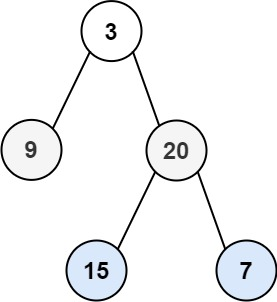
\includegraphics{896b03ec-fa75-4b76-b0de-69d3f23f255c.jpg}

\begin{itemize}
\tightlist
\item
  Input: root = {[}3,9,20,null,null,15,7{]}
\item
  Output: {[}{[}3{]},{[}9,20{]},{[}15,7{]}{]}
\end{itemize}

\textbf{Example 2:}

\begin{itemize}
\tightlist
\item
  Input: root = {[}1{]}
\item
  Output: {[}{[}1{]}{]}
\end{itemize}

\textbf{Example 3:}

\begin{itemize}
\tightlist
\item
  Input: root = {[}{]}
\item
  Output: {[}{]}
\end{itemize}

    \subsubsection{Q102. pseudocode}\label{q102.-pseudocode}

    \begin{tcolorbox}[breakable, size=fbox, boxrule=1pt, pad at break*=1mm,colback=cellbackground, colframe=cellborder]
\prompt{In}{incolor}{ }{\boxspacing}
\begin{Verbatim}[commandchars=\\\{\}]
\PY{n}{function} \PY{n}{level\PYZus{}order}\PY{p}{(}\PY{n}{root}\PY{p}{)}
\PY{k}{if} \PY{n}{root} \PY{o+ow}{is} \PY{n}{null}
    \PY{k}{return} \PY{n}{empty} \PY{n+nb}{list}
\PY{n}{initialize} \PY{n}{empty} \PY{n+nb}{list} \PY{n}{ans}
\PY{n}{initialize} \PY{n}{deque} \PY{k}{with} \PY{n}{root}
\PY{k}{while} \PY{n}{deque} \PY{o+ow}{is} \PY{o+ow}{not} \PY{n}{empty}
    \PY{n}{initialize} \PY{n}{empty} \PY{n+nb}{list} \PY{n}{vals}
    \PY{k}{for} \PY{n}{each} \PY{n}{element} \PY{o+ow}{in} \PY{n}{deque}
        \PY{n}{remove} \PY{n}{node} \PY{k+kn}{from} \PY{n+nn}{deque}
        \PY{n}{append} \PY{n}{node}\PY{o}{.}\PY{n}{val} \PY{n}{to} \PY{n}{vals}
        \PY{k}{if} \PY{n}{node}\PY{o}{.}\PY{n}{left} \PY{o+ow}{is} \PY{o+ow}{not} \PY{n}{null}\PY{p}{,} \PY{n}{append} \PY{n}{node}\PY{o}{.}\PY{n}{left} \PY{n}{to} \PY{n}{deque}
        \PY{k}{if} \PY{n}{node}\PY{o}{.}\PY{n}{right} \PY{o+ow}{is} \PY{o+ow}{not} \PY{n}{null}\PY{p}{,} \PY{n}{append} \PY{n}{node}\PY{o}{.}\PY{n}{right} \PY{n}{to} \PY{n}{deque}
    \PY{n}{append} \PY{n}{vals} \PY{n}{to} \PY{n}{ans}
\PY{k}{return} \PY{n}{ans}
\end{Verbatim}
\end{tcolorbox}

    \subsubsection{Q102 code.py}\label{q102-code.py}

    \begin{tcolorbox}[breakable, size=fbox, boxrule=1pt, pad at break*=1mm,colback=cellbackground, colframe=cellborder]
\prompt{In}{incolor}{14}{\boxspacing}
\begin{Verbatim}[commandchars=\\\{\}]
\PY{k+kn}{from} \PY{n+nn}{typing} \PY{k+kn}{import} \PY{n}{List}\PY{p}{,} \PY{n}{Optional}
\PY{k+kn}{from} \PY{n+nn}{collections} \PY{k+kn}{import} \PY{n}{deque}

\PY{k}{class} \PY{n+nc}{TreeNode}\PY{p}{:}
    \PY{k}{def} \PY{n+nf+fm}{\PYZus{}\PYZus{}init\PYZus{}\PYZus{}}\PY{p}{(}\PY{n+nb+bp}{self}\PY{p}{,} \PY{n}{val}\PY{o}{=}\PY{l+m+mi}{0}\PY{p}{,} \PY{n}{left}\PY{o}{=}\PY{k+kc}{None}\PY{p}{,} \PY{n}{right}\PY{o}{=}\PY{k+kc}{None}\PY{p}{)}\PY{p}{:}
        \PY{n+nb+bp}{self}\PY{o}{.}\PY{n}{val} \PY{o}{=} \PY{n}{val}
        \PY{n+nb+bp}{self}\PY{o}{.}\PY{n}{left} \PY{o}{=} \PY{n}{left}
        \PY{n+nb+bp}{self}\PY{o}{.}\PY{n}{right} \PY{o}{=} \PY{n}{right}

\PY{k}{class} \PY{n+nc}{Solution}\PY{p}{:}
    \PY{k}{def} \PY{n+nf}{levelOrder}\PY{p}{(}\PY{n+nb+bp}{self}\PY{p}{,} \PY{n}{root}\PY{p}{:} \PY{n}{Optional}\PY{p}{[}\PY{n}{TreeNode}\PY{p}{]}\PY{p}{)} \PY{o}{\PYZhy{}}\PY{o}{\PYZgt{}} \PY{n}{List}\PY{p}{[}\PY{n}{List}\PY{p}{[}\PY{n+nb}{int}\PY{p}{]}\PY{p}{]}\PY{p}{:}
        \PY{k}{if} \PY{n}{root} \PY{o+ow}{is} \PY{k+kc}{None}\PY{p}{:}
            \PY{k}{return} \PY{p}{[}\PY{p}{]}
        \PY{n}{ans} \PY{o}{=} \PY{p}{[}\PY{p}{]}
        \PY{n}{q} \PY{o}{=} \PY{n}{deque}\PY{p}{(}\PY{p}{[}\PY{n}{root}\PY{p}{]}\PY{p}{)}
        \PY{k}{while} \PY{n}{q}\PY{p}{:}
            \PY{n}{vals} \PY{o}{=} \PY{p}{[}\PY{p}{]}
            \PY{k}{for} \PY{n}{\PYZus{}} \PY{o+ow}{in} \PY{n+nb}{range}\PY{p}{(}\PY{n+nb}{len}\PY{p}{(}\PY{n}{q}\PY{p}{)}\PY{p}{)}\PY{p}{:}
                \PY{n}{node} \PY{o}{=} \PY{n}{q}\PY{o}{.}\PY{n}{popleft}\PY{p}{(}\PY{p}{)}
                \PY{n}{vals}\PY{o}{.}\PY{n}{append}\PY{p}{(}\PY{n}{node}\PY{o}{.}\PY{n}{val}\PY{p}{)}
                \PY{k}{if} \PY{n}{node}\PY{o}{.}\PY{n}{left}\PY{p}{:}
                    \PY{n}{q}\PY{o}{.}\PY{n}{append}\PY{p}{(}\PY{n}{node}\PY{o}{.}\PY{n}{left}\PY{p}{)}
                \PY{k}{if} \PY{n}{node}\PY{o}{.}\PY{n}{right}\PY{p}{:}
                    \PY{n}{q}\PY{o}{.}\PY{n}{append}\PY{p}{(}\PY{n}{node}\PY{o}{.}\PY{n}{right}\PY{p}{)}
            \PY{n}{ans}\PY{o}{.}\PY{n}{append}\PY{p}{(}\PY{n}{vals}\PY{p}{)}
        \PY{k}{return} \PY{n}{ans}


\PY{n}{root} \PY{o}{=} \PY{n}{TreeNode}\PY{p}{(}\PY{l+m+mi}{3}\PY{p}{)}
\PY{n}{root}\PY{o}{.}\PY{n}{left} \PY{o}{=} \PY{n}{TreeNode}\PY{p}{(}\PY{l+m+mi}{9}\PY{p}{)}
\PY{n}{root}\PY{o}{.}\PY{n}{right} \PY{o}{=} \PY{n}{TreeNode}\PY{p}{(}\PY{l+m+mi}{20}\PY{p}{)}
\PY{n}{root}\PY{o}{.}\PY{n}{right}\PY{o}{.}\PY{n}{left} \PY{o}{=} \PY{n}{TreeNode}\PY{p}{(}\PY{l+m+mi}{15}\PY{p}{)}
\PY{n}{root}\PY{o}{.}\PY{n}{right}\PY{o}{.}\PY{n}{right} \PY{o}{=} \PY{n}{TreeNode}\PY{p}{(}\PY{l+m+mi}{7}\PY{p}{)}

\PY{n}{solution} \PY{o}{=} \PY{n}{Solution}\PY{p}{(}\PY{p}{)}
\PY{n}{output} \PY{o}{=} \PY{n}{solution}\PY{o}{.}\PY{n}{levelOrder}\PY{p}{(}\PY{n}{root}\PY{p}{)}
\PY{n+nb}{print}\PY{p}{(}\PY{n}{output}\PY{p}{)} 
\end{Verbatim}
\end{tcolorbox}

    \begin{Verbatim}[commandchars=\\\{\}]
[[3], [9, 20], [15, 7]]
    \end{Verbatim}

    \textbf{Problem5-LeetcodeQ 199-Binary Tree Right Side View-Medium}

\begin{figure}
\centering
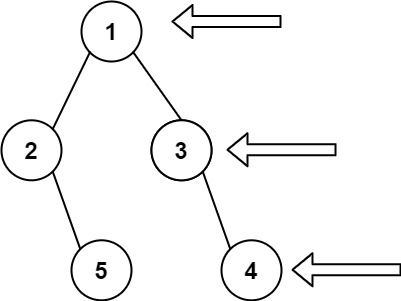
\includegraphics{a754605f-016a-4c9e-b9d7-c79ca5b59a2f.jpg}
\caption{tree3.jpg}
\end{figure}

\textbf{Example 1:} - Input: root = {[}1,2,3,null,5,null,4{]} - Output:
{[}1,3,4{]}

\textbf{Example 2:}

\begin{itemize}
\tightlist
\item
  Input: root = {[}1,null,3{]}
\item
  Output: {[}1,3{]}
\end{itemize}

\textbf{Example 3:}

\begin{itemize}
\tightlist
\item
  Input: root = {[}{]}
\item
  Output: {[}{]}
\end{itemize}

    \subsubsection{Q199. pseudocode}\label{q199.-pseudocode}

    \begin{tcolorbox}[breakable, size=fbox, boxrule=1pt, pad at break*=1mm,colback=cellbackground, colframe=cellborder]
\prompt{In}{incolor}{ }{\boxspacing}
\begin{Verbatim}[commandchars=\\\{\}]
\PY{n}{function} \PY{n}{right\PYZus{}side\PYZus{}view}\PY{p}{(}\PY{n}{root}\PY{p}{)}
\PY{n}{initialize} \PY{n}{empty} \PY{n+nb}{list} \PY{n}{res}
\PY{n}{define} \PY{n}{inner} \PY{n}{function} \PY{n}{dfs}\PY{p}{(}\PY{n}{root}\PY{p}{,} \PY{n}{depth}\PY{p}{)}
    \PY{k}{if} \PY{n}{root} \PY{o+ow}{is} \PY{n}{null}\PY{p}{,} \PY{k}{return}
    \PY{k}{if} \PY{n}{length} \PY{n}{of} \PY{n}{res} \PY{o+ow}{is} \PY{n}{less} \PY{n}{than} \PY{o+ow}{or} \PY{n}{equal} \PY{n}{to} \PY{n}{depth}
        \PY{n}{append} \PY{l+m+mi}{0} \PY{n}{to} \PY{n}{res}
    \PY{n+nb}{set} \PY{n}{res}\PY{p}{[}\PY{n}{depth}\PY{p}{]} \PY{n}{to} \PY{n}{root}\PY{o}{.}\PY{n}{val}
    \PY{n}{call} \PY{n}{dfs}\PY{p}{(}\PY{n}{root}\PY{o}{.}\PY{n}{left}\PY{p}{,} \PY{n}{depth} \PY{o}{+} \PY{l+m+mi}{1}\PY{p}{)}
    \PY{n}{call} \PY{n}{dfs}\PY{p}{(}\PY{n}{root}\PY{o}{.}\PY{n}{right}\PY{p}{,} \PY{n}{depth} \PY{o}{+} \PY{l+m+mi}{1}\PY{p}{)}
\PY{n}{call} \PY{n}{dfs} \PY{k}{with} \PY{n}{root} \PY{o+ow}{and} \PY{n}{depth} \PY{l+m+mi}{0}
\PY{k}{return} \PY{n}{res}
\end{Verbatim}
\end{tcolorbox}

    \subsubsection{Q199. code.py}\label{q199.-code.py}

    \begin{tcolorbox}[breakable, size=fbox, boxrule=1pt, pad at break*=1mm,colback=cellbackground, colframe=cellborder]
\prompt{In}{incolor}{20}{\boxspacing}
\begin{Verbatim}[commandchars=\\\{\}]
\PY{k+kn}{from} \PY{n+nn}{typing} \PY{k+kn}{import} \PY{n}{List}\PY{p}{,} \PY{n}{Optional}

\PY{k}{class} \PY{n+nc}{TreeNode}\PY{p}{:}
    \PY{k}{def} \PY{n+nf+fm}{\PYZus{}\PYZus{}init\PYZus{}\PYZus{}}\PY{p}{(}\PY{n+nb+bp}{self}\PY{p}{,} \PY{n}{val}\PY{o}{=}\PY{l+m+mi}{0}\PY{p}{,} \PY{n}{left}\PY{o}{=}\PY{k+kc}{None}\PY{p}{,} \PY{n}{right}\PY{o}{=}\PY{k+kc}{None}\PY{p}{)}\PY{p}{:}
        \PY{n+nb+bp}{self}\PY{o}{.}\PY{n}{val} \PY{o}{=} \PY{n}{val}
        \PY{n+nb+bp}{self}\PY{o}{.}\PY{n}{left} \PY{o}{=} \PY{n}{left}
        \PY{n+nb+bp}{self}\PY{o}{.}\PY{n}{right} \PY{o}{=} \PY{n}{right}

\PY{k}{class} \PY{n+nc}{Solution}\PY{p}{:}
    \PY{k}{def} \PY{n+nf}{rightSideView}\PY{p}{(}\PY{n+nb+bp}{self}\PY{p}{,} \PY{n}{root}\PY{p}{:} \PY{n}{Optional}\PY{p}{[}\PY{n}{TreeNode}\PY{p}{]}\PY{p}{)} \PY{o}{\PYZhy{}}\PY{o}{\PYZgt{}} \PY{n}{List}\PY{p}{[}\PY{n+nb}{int}\PY{p}{]}\PY{p}{:}
        \PY{n}{res} \PY{o}{=} \PY{p}{[}\PY{p}{]}
        \PY{k}{def} \PY{n+nf}{dfs}\PY{p}{(}\PY{n}{root}\PY{p}{,} \PY{n}{depth}\PY{p}{)}\PY{p}{:}
            \PY{k}{if} \PY{o+ow}{not} \PY{n}{root}\PY{p}{:}
                \PY{k}{return}
            \PY{k}{if} \PY{n+nb}{len}\PY{p}{(}\PY{n}{res}\PY{p}{)} \PY{o}{\PYZlt{}}\PY{o}{=} \PY{n}{depth}\PY{p}{:}
                \PY{n}{res}\PY{o}{.}\PY{n}{append}\PY{p}{(}\PY{l+m+mi}{0}\PY{p}{)}
            \PY{n}{res}\PY{p}{[}\PY{n}{depth}\PY{p}{]} \PY{o}{=} \PY{n}{root}\PY{o}{.}\PY{n}{val}
            \PY{n}{dfs}\PY{p}{(}\PY{n}{root}\PY{o}{.}\PY{n}{left}\PY{p}{,} \PY{n}{depth} \PY{o}{+} \PY{l+m+mi}{1}\PY{p}{)}
            \PY{n}{dfs}\PY{p}{(}\PY{n}{root}\PY{o}{.}\PY{n}{right}\PY{p}{,} \PY{n}{depth} \PY{o}{+} \PY{l+m+mi}{1}\PY{p}{)}

        \PY{n}{dfs}\PY{p}{(}\PY{n}{root}\PY{p}{,} \PY{l+m+mi}{0}\PY{p}{)}
        \PY{k}{return} \PY{n}{res}


\PY{k+kn}{from} \PY{n+nn}{collections} \PY{k+kn}{import} \PY{n}{deque}

\PY{k}{def} \PY{n+nf}{print\PYZus{}tree}\PY{p}{(}\PY{n}{root}\PY{p}{)}\PY{p}{:}
    \PY{k}{if} \PY{o+ow}{not} \PY{n}{root}\PY{p}{:}
        \PY{k}{return} \PY{p}{[}\PY{p}{]}
    \PY{n}{result} \PY{o}{=} \PY{p}{[}\PY{p}{]}
    \PY{n}{queue} \PY{o}{=} \PY{n}{deque}\PY{p}{(}\PY{p}{[}\PY{n}{root}\PY{p}{]}\PY{p}{)}
    \PY{k}{while} \PY{n}{queue}\PY{p}{:}
        \PY{n}{node} \PY{o}{=} \PY{n}{queue}\PY{o}{.}\PY{n}{popleft}\PY{p}{(}\PY{p}{)}
        \PY{k}{if} \PY{n}{node}\PY{p}{:}
            \PY{n}{result}\PY{o}{.}\PY{n}{append}\PY{p}{(}\PY{n}{node}\PY{o}{.}\PY{n}{val}\PY{p}{)}
            \PY{n}{queue}\PY{o}{.}\PY{n}{append}\PY{p}{(}\PY{n}{node}\PY{o}{.}\PY{n}{left}\PY{p}{)}
            \PY{n}{queue}\PY{o}{.}\PY{n}{append}\PY{p}{(}\PY{n}{node}\PY{o}{.}\PY{n}{right}\PY{p}{)}
        \PY{k}{else}\PY{p}{:}
            \PY{n}{result}\PY{o}{.}\PY{n}{append}\PY{p}{(}\PY{k+kc}{None}\PY{p}{)}
    \PY{c+c1}{\PYZsh{} Remove trailing None values}
    \PY{k}{while} \PY{n}{result} \PY{o+ow}{and} \PY{n}{result}\PY{p}{[}\PY{o}{\PYZhy{}}\PY{l+m+mi}{1}\PY{p}{]} \PY{o+ow}{is} \PY{k+kc}{None}\PY{p}{:}
        \PY{n}{result}\PY{o}{.}\PY{n}{pop}\PY{p}{(}\PY{p}{)}
    \PY{k}{return} \PY{n}{result}


\PY{n}{root} \PY{o}{=} \PY{n}{TreeNode}\PY{p}{(}\PY{l+m+mi}{1}\PY{p}{)}
\PY{n}{root}\PY{o}{.}\PY{n}{left} \PY{o}{=} \PY{n}{TreeNode}\PY{p}{(}\PY{l+m+mi}{2}\PY{p}{)}
\PY{n}{root}\PY{o}{.}\PY{n}{right} \PY{o}{=} \PY{n}{TreeNode}\PY{p}{(}\PY{l+m+mi}{3}\PY{p}{)}
\PY{n}{root}\PY{o}{.}\PY{n}{left}\PY{o}{.}\PY{n}{right} \PY{o}{=} \PY{n}{TreeNode}\PY{p}{(}\PY{l+m+mi}{5}\PY{p}{)}
\PY{n}{root}\PY{o}{.}\PY{n}{right}\PY{o}{.}\PY{n}{right} \PY{o}{=} \PY{n}{TreeNode}\PY{p}{(}\PY{l+m+mi}{4}\PY{p}{)}

\PY{c+c1}{\PYZsh{} Creating an instance of Solution and testing the method}
\PY{n}{solution} \PY{o}{=} \PY{n}{Solution}\PY{p}{(}\PY{p}{)}
\PY{n}{output} \PY{o}{=} \PY{n}{solution}\PY{o}{.}\PY{n}{rightSideView}\PY{p}{(}\PY{n}{root}\PY{p}{)}
\PY{n+nb}{print}\PY{p}{(}\PY{n}{output}\PY{p}{)}  
\end{Verbatim}
\end{tcolorbox}

    \begin{Verbatim}[commandchars=\\\{\}]
[1, 3, 4]
    \end{Verbatim}

    \textbf{Problem6-LeetcodeQ 112-Path Sum-Easy}

Given the root of a binary tree and an integer targetSum, return true if
the tree has a root-to-leaf path such that adding up all the values
along the path equals targetSum.

A *\textbf{leaf} is a node with no children.

\textbf{Example 1:}

\begin{figure}
\centering
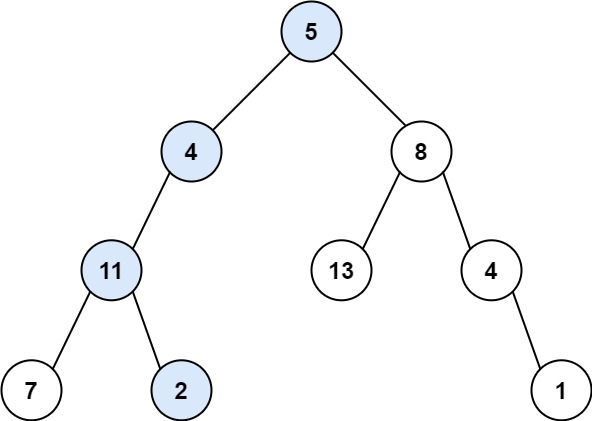
\includegraphics{ee18dc1e-61f4-4b2b-8045-58f649d8d464.jpg}
\caption{pathsum1.jpg}
\end{figure}

\begin{itemize}
\tightlist
\item
  Input: root = {[}5,4,8,11,null,13,4,7,2,null,null,null,1{]}, targetSum
  = 22
\item
  Output: true
\item
  Explanation: The root-to-leaf path with the target sum is shown.
\end{itemize}

\textbf{Example 2:}

\begin{figure}
\centering
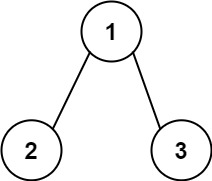
\includegraphics{14094bf8-292d-4f6a-ad02-aa79df01c609.jpg}
\caption{pathsum2.jpg}
\end{figure}

\begin{itemize}
\tightlist
\item
  Input: root = {[}1,2,3{]}, targetSum = 5
\item
  Output: false
\item
  Explanation: There two root-to-leaf paths in the tree:
\item
  \begin{itemize}
  \tightlist
  \item
    (1 --\textgreater{} 2): The sum is 3.
  \end{itemize}
\item
  \begin{itemize}
  \tightlist
  \item
    (1 --\textgreater{} 3): The sum is 4.
  \end{itemize}
\item
  \begin{itemize}
  \tightlist
  \item
    There is no root-to-leaf path with sum = 5.
  \end{itemize}
\end{itemize}

\textbf{Example 3:}

\begin{itemize}
\tightlist
\item
  Input: root = {[}{]}, targetSum = 0
\item
  Output: false
\item
  Explanation: Since the tree is empty, there are no root-to-leaf paths.
\end{itemize}

    \subsubsection{Q112. pseudocode}\label{q112.-pseudocode}

    \begin{tcolorbox}[breakable, size=fbox, boxrule=1pt, pad at break*=1mm,colback=cellbackground, colframe=cellborder]
\prompt{In}{incolor}{ }{\boxspacing}
\begin{Verbatim}[commandchars=\\\{\}]
\PY{n}{function} \PY{n}{has\PYZus{}path\PYZus{}sum}\PY{p}{(}\PY{n}{root}\PY{p}{,} \PY{n}{target\PYZus{}sum}\PY{p}{)}
\PY{k}{if} \PY{n}{root} \PY{o+ow}{is} \PY{n}{null}
    \PY{k}{return} \PY{n}{false}
\PY{n}{subtract} \PY{n}{root}\PY{o}{.}\PY{n}{val} \PY{k+kn}{from} \PY{n+nn}{target\PYZus{}sum}
\PY{k}{if} \PY{n}{root}\PY{o}{.}\PY{n}{left} \PY{o+ow}{is} \PY{n}{null} \PY{o+ow}{and} \PY{n}{root}\PY{o}{.}\PY{n}{right} \PY{o+ow}{is} \PY{n}{null}
    \PY{k}{return} \PY{n}{target\PYZus{}sum} \PY{o+ow}{is} \PY{n}{equal} \PY{n}{to} \PY{l+m+mi}{0}
\PY{k}{return} \PY{n}{has\PYZus{}path\PYZus{}sum}\PY{p}{(}\PY{n}{root}\PY{o}{.}\PY{n}{left}\PY{p}{,} \PY{n}{target\PYZus{}sum}\PY{p}{)} \PY{o+ow}{or} \PY{n}{has\PYZus{}path\PYZus{}sum}\PY{p}{(}\PY{n}{root}\PY{o}{.}\PY{n}{right}\PY{p}{,} \PY{n}{target\PYZus{}sum}\PY{p}{)}
\end{Verbatim}
\end{tcolorbox}

    \subsubsection{Q112. code.py}\label{q112.-code.py}

    \begin{tcolorbox}[breakable, size=fbox, boxrule=1pt, pad at break*=1mm,colback=cellbackground, colframe=cellborder]
\prompt{In}{incolor}{24}{\boxspacing}
\begin{Verbatim}[commandchars=\\\{\}]
\PY{k+kn}{from} \PY{n+nn}{typing} \PY{k+kn}{import} \PY{n}{Optional}

\PY{k}{class} \PY{n+nc}{TreeNode}\PY{p}{:}
    \PY{k}{def} \PY{n+nf+fm}{\PYZus{}\PYZus{}init\PYZus{}\PYZus{}}\PY{p}{(}\PY{n+nb+bp}{self}\PY{p}{,} \PY{n}{val}\PY{o}{=}\PY{l+m+mi}{0}\PY{p}{,} \PY{n}{left}\PY{o}{=}\PY{k+kc}{None}\PY{p}{,} \PY{n}{right}\PY{o}{=}\PY{k+kc}{None}\PY{p}{)}\PY{p}{:}
        \PY{n+nb+bp}{self}\PY{o}{.}\PY{n}{val} \PY{o}{=} \PY{n}{val}
        \PY{n+nb+bp}{self}\PY{o}{.}\PY{n}{left} \PY{o}{=} \PY{n}{left}
        \PY{n+nb+bp}{self}\PY{o}{.}\PY{n}{right} \PY{o}{=} \PY{n}{right}

\PY{k}{class} \PY{n+nc}{Solution}\PY{p}{:}
    \PY{k}{def} \PY{n+nf}{hasPathSum}\PY{p}{(}\PY{n+nb+bp}{self}\PY{p}{,} \PY{n}{root}\PY{p}{:} \PY{n}{Optional}\PY{p}{[}\PY{n}{TreeNode}\PY{p}{]}\PY{p}{,} \PY{n}{targetSum}\PY{p}{:} \PY{n+nb}{int}\PY{p}{)} \PY{o}{\PYZhy{}}\PY{o}{\PYZgt{}} \PY{n+nb}{bool}\PY{p}{:}
        \PY{k}{if} \PY{n}{root} \PY{o+ow}{is} \PY{k+kc}{None}\PY{p}{:}
            \PY{k}{return} \PY{k+kc}{False}
        \PY{n}{targetSum} \PY{o}{\PYZhy{}}\PY{o}{=} \PY{n}{root}\PY{o}{.}\PY{n}{val}
        \PY{k}{if} \PY{n}{root}\PY{o}{.}\PY{n}{left} \PY{o+ow}{is} \PY{k+kc}{None} \PY{o+ow}{and} \PY{n}{root}\PY{o}{.}\PY{n}{right} \PY{o+ow}{is} \PY{k+kc}{None}\PY{p}{:}
            \PY{k}{return} \PY{n}{targetSum} \PY{o}{==} \PY{l+m+mi}{0}
        \PY{k}{return} \PY{n+nb+bp}{self}\PY{o}{.}\PY{n}{hasPathSum}\PY{p}{(}\PY{n}{root}\PY{o}{.}\PY{n}{left}\PY{p}{,} \PY{n}{targetSum}\PY{p}{)} \PY{o+ow}{or} \PY{n+nb+bp}{self}\PY{o}{.}\PY{n}{hasPathSum}\PY{p}{(}\PY{n}{root}\PY{o}{.}\PY{n}{right}\PY{p}{,} \PY{n}{targetSum}\PY{p}{)}


\PY{k+kn}{from} \PY{n+nn}{collections} \PY{k+kn}{import} \PY{n}{deque}

\PY{k}{def} \PY{n+nf}{print\PYZus{}tree}\PY{p}{(}\PY{n}{root}\PY{p}{)}\PY{p}{:}
    \PY{k}{if} \PY{o+ow}{not} \PY{n}{root}\PY{p}{:}
        \PY{k}{return} \PY{p}{[}\PY{p}{]}
    \PY{n}{result} \PY{o}{=} \PY{p}{[}\PY{p}{]}
    \PY{n}{queue} \PY{o}{=} \PY{n}{deque}\PY{p}{(}\PY{p}{[}\PY{n}{root}\PY{p}{]}\PY{p}{)}
    \PY{k}{while} \PY{n}{queue}\PY{p}{:}
        \PY{n}{node} \PY{o}{=} \PY{n}{queue}\PY{o}{.}\PY{n}{popleft}\PY{p}{(}\PY{p}{)}
        \PY{k}{if} \PY{n}{node}\PY{p}{:}
            \PY{n}{result}\PY{o}{.}\PY{n}{append}\PY{p}{(}\PY{n}{node}\PY{o}{.}\PY{n}{val}\PY{p}{)}
            \PY{n}{queue}\PY{o}{.}\PY{n}{append}\PY{p}{(}\PY{n}{node}\PY{o}{.}\PY{n}{left}\PY{p}{)}
            \PY{n}{queue}\PY{o}{.}\PY{n}{append}\PY{p}{(}\PY{n}{node}\PY{o}{.}\PY{n}{right}\PY{p}{)}
        \PY{k}{else}\PY{p}{:}
            \PY{n}{result}\PY{o}{.}\PY{n}{append}\PY{p}{(}\PY{k+kc}{None}\PY{p}{)}
    \PY{c+c1}{\PYZsh{} Remove trailing None values}
    \PY{k}{while} \PY{n}{result} \PY{o+ow}{and} \PY{n}{result}\PY{p}{[}\PY{o}{\PYZhy{}}\PY{l+m+mi}{1}\PY{p}{]} \PY{o+ow}{is} \PY{k+kc}{None}\PY{p}{:}
        \PY{n}{result}\PY{o}{.}\PY{n}{pop}\PY{p}{(}\PY{p}{)}
    \PY{k}{return} \PY{n}{result}


\PY{n}{root} \PY{o}{=} \PY{n}{TreeNode}\PY{p}{(}\PY{l+m+mi}{5}\PY{p}{)}
\PY{n}{root}\PY{o}{.}\PY{n}{left} \PY{o}{=} \PY{n}{TreeNode}\PY{p}{(}\PY{l+m+mi}{4}\PY{p}{)}
\PY{n}{root}\PY{o}{.}\PY{n}{right} \PY{o}{=} \PY{n}{TreeNode}\PY{p}{(}\PY{l+m+mi}{8}\PY{p}{)}
\PY{n}{root}\PY{o}{.}\PY{n}{left}\PY{o}{.}\PY{n}{left} \PY{o}{=} \PY{n}{TreeNode}\PY{p}{(}\PY{l+m+mi}{11}\PY{p}{)}
\PY{n}{root}\PY{o}{.}\PY{n}{left}\PY{o}{.}\PY{n}{left}\PY{o}{.}\PY{n}{left} \PY{o}{=} \PY{n}{TreeNode}\PY{p}{(}\PY{l+m+mi}{7}\PY{p}{)}
\PY{n}{root}\PY{o}{.}\PY{n}{left}\PY{o}{.}\PY{n}{left}\PY{o}{.}\PY{n}{right} \PY{o}{=} \PY{n}{TreeNode}\PY{p}{(}\PY{l+m+mi}{2}\PY{p}{)}
\PY{n}{root}\PY{o}{.}\PY{n}{right}\PY{o}{.}\PY{n}{left} \PY{o}{=} \PY{n}{TreeNode}\PY{p}{(}\PY{l+m+mi}{13}\PY{p}{)}
\PY{n}{root}\PY{o}{.}\PY{n}{right}\PY{o}{.}\PY{n}{right} \PY{o}{=} \PY{n}{TreeNode}\PY{p}{(}\PY{l+m+mi}{4}\PY{p}{)}
\PY{n}{root}\PY{o}{.}\PY{n}{right}\PY{o}{.}\PY{n}{right}\PY{o}{.}\PY{n}{right} \PY{o}{=} \PY{n}{TreeNode}\PY{p}{(}\PY{l+m+mi}{1}\PY{p}{)}

\PY{n}{solution} \PY{o}{=} \PY{n}{Solution}\PY{p}{(}\PY{p}{)}
\PY{n}{output} \PY{o}{=} \PY{n}{solution}\PY{o}{.}\PY{n}{hasPathSum}\PY{p}{(}\PY{n}{root}\PY{p}{,} \PY{l+m+mi}{22}\PY{p}{)}
\PY{n+nb}{print}\PY{p}{(}\PY{n}{output}\PY{p}{)}  
\end{Verbatim}
\end{tcolorbox}

    \begin{Verbatim}[commandchars=\\\{\}]
True
    \end{Verbatim}

    \textbf{Problem7-LeetcodeQ 78-Subsets-Medium}

Given an integer array nums of unique elements, return all possible
subsets (the power set).

The solution set must not contain duplicate subsets. Return the solution
in any order.

\textbf{Example 1:}

\begin{itemize}
\tightlist
\item
  Input: nums = {[}1,2,3{]}
\item
  Output:
  {[}{[}{]},{[}1{]},{[}2{]},{[}1,2{]},{[}3{]},{[}1,3{]},{[}2,3{]},{[}1,2,3{]}{]}
\end{itemize}

\textbf{Example 2:}

\begin{itemize}
\tightlist
\item
  Input: nums = {[}0{]}
\item
  Output: {[}{[}{]},{[}0{]}{]}
\end{itemize}

Note: All the numbers of nums are \textbf{unique}.

    \subsubsection{Q78. pseudocode}\label{q78.-pseudocode}

    \begin{tcolorbox}[breakable, size=fbox, boxrule=1pt, pad at break*=1mm,colback=cellbackground, colframe=cellborder]
\prompt{In}{incolor}{ }{\boxspacing}
\begin{Verbatim}[commandchars=\\\{\}]
\PY{n}{function} \PY{n}{subsets}\PY{p}{(}\PY{n}{nums}\PY{p}{)}
\PY{n}{initialize} \PY{n}{empty} \PY{n+nb}{list} \PY{n}{ans}
\PY{n}{initialize} \PY{n}{empty} \PY{n+nb}{list} \PY{n}{path}
\PY{n+nb}{set} \PY{n}{n} \PY{n}{to} \PY{n}{length} \PY{n}{of} \PY{n}{nums}

\PY{n}{define} \PY{n}{inner} \PY{n}{function} \PY{n}{dfs}\PY{p}{(}\PY{n}{i}\PY{p}{)}
    \PY{k}{if} \PY{n}{i} \PY{o+ow}{is} \PY{n}{equal} \PY{n}{to} \PY{n}{n}
        \PY{n}{append} \PY{n}{a} \PY{n}{copy} \PY{n}{of} \PY{n}{path} \PY{n}{to} \PY{n}{ans}
        \PY{k}{return}
    \PY{n}{call} \PY{n}{dfs}\PY{p}{(}\PY{n}{i} \PY{o}{+} \PY{l+m+mi}{1}\PY{p}{)}
    \PY{n}{append} \PY{n}{nums}\PY{p}{[}\PY{n}{i}\PY{p}{]} \PY{n}{to} \PY{n}{path}
    \PY{n}{call} \PY{n}{dfs}\PY{p}{(}\PY{n}{i} \PY{o}{+} \PY{l+m+mi}{1}\PY{p}{)}
    \PY{n}{remove} \PY{n}{the} \PY{n}{last} \PY{n}{element} \PY{k+kn}{from} \PY{n+nn}{path}

\PY{n}{call} \PY{n}{dfs}\PY{p}{(}\PY{l+m+mi}{0}\PY{p}{)}
\PY{k}{return} \PY{n}{ans}

\PY{c+c1}{\PYZsh{}\PYZsh{}\PYZsh{}\PYZsh{}\PYZsh{}\PYZsh{}\PYZsh{}\PYZsh{}\PYZsh{}\PYZsh{}\PYZsh{}\PYZsh{}\PYZsh{}\PYZsh{}\PYZsh{}\PYZsh{}\PYZsh{}\PYZsh{}\PYZsh{}\PYZsh{}\PYZsh{}\PYZsh{}\PYZsh{}}
\PY{n}{ans} \PY{o+ow}{is} \PY{n}{the} \PY{n+nb}{list} \PY{n}{of} \PY{n+nb}{all} \PY{n}{subsets} \PY{n}{to} \PY{n}{be} \PY{n}{returned}\PY{o}{.}
\PY{n}{path} \PY{o+ow}{is} \PY{n}{the} \PY{n}{current} \PY{n}{subset} \PY{n}{being} \PY{n}{constructed}\PY{o}{.}
\end{Verbatim}
\end{tcolorbox}

    \subsubsection{Q78. code.py}\label{q78.-code.py}

    \begin{tcolorbox}[breakable, size=fbox, boxrule=1pt, pad at break*=1mm,colback=cellbackground, colframe=cellborder]
\prompt{In}{incolor}{27}{\boxspacing}
\begin{Verbatim}[commandchars=\\\{\}]
\PY{k+kn}{from} \PY{n+nn}{typing} \PY{k+kn}{import} \PY{n}{List}

\PY{k}{class} \PY{n+nc}{Solution}\PY{p}{:}
    \PY{k}{def} \PY{n+nf}{subsets}\PY{p}{(}\PY{n+nb+bp}{self}\PY{p}{,} \PY{n}{nums}\PY{p}{:} \PY{n}{List}\PY{p}{[}\PY{n+nb}{int}\PY{p}{]}\PY{p}{)} \PY{o}{\PYZhy{}}\PY{o}{\PYZgt{}} \PY{n}{List}\PY{p}{[}\PY{n}{List}\PY{p}{[}\PY{n+nb}{int}\PY{p}{]}\PY{p}{]}\PY{p}{:}
        \PY{n}{ans} \PY{o}{=} \PY{p}{[}\PY{p}{]}
        \PY{n}{path} \PY{o}{=} \PY{p}{[}\PY{p}{]}
        \PY{n}{n} \PY{o}{=} \PY{n+nb}{len}\PY{p}{(}\PY{n}{nums}\PY{p}{)}

        \PY{k}{def} \PY{n+nf}{dfs}\PY{p}{(}\PY{n}{i}\PY{p}{:} \PY{n+nb}{int}\PY{p}{)} \PY{o}{\PYZhy{}}\PY{o}{\PYZgt{}} \PY{k+kc}{None}\PY{p}{:}
            \PY{k}{if} \PY{n}{i} \PY{o}{==} \PY{n}{n}\PY{p}{:}
                \PY{n}{ans}\PY{o}{.}\PY{n}{append}\PY{p}{(}\PY{n}{path}\PY{o}{.}\PY{n}{copy}\PY{p}{(}\PY{p}{)}\PY{p}{)}
                \PY{k}{return}
            \PY{n}{dfs}\PY{p}{(}\PY{n}{i} \PY{o}{+} \PY{l+m+mi}{1}\PY{p}{)}
            \PY{n}{path}\PY{o}{.}\PY{n}{append}\PY{p}{(}\PY{n}{nums}\PY{p}{[}\PY{n}{i}\PY{p}{]}\PY{p}{)}
            \PY{n}{dfs}\PY{p}{(}\PY{n}{i} \PY{o}{+} \PY{l+m+mi}{1}\PY{p}{)}
            \PY{n}{path}\PY{o}{.}\PY{n}{pop}\PY{p}{(}\PY{p}{)}

        \PY{n}{dfs}\PY{p}{(}\PY{l+m+mi}{0}\PY{p}{)}
        \PY{k}{return} \PY{n}{ans}


\PY{n}{nums} \PY{o}{=} \PY{p}{[}\PY{l+m+mi}{1}\PY{p}{,} \PY{l+m+mi}{2}\PY{p}{,} \PY{l+m+mi}{3}\PY{p}{]}
\PY{n}{solution} \PY{o}{=} \PY{n}{Solution}\PY{p}{(}\PY{p}{)}
\PY{n}{output} \PY{o}{=} \PY{n}{solution}\PY{o}{.}\PY{n}{subsets}\PY{p}{(}\PY{n}{nums}\PY{p}{)}
\PY{n+nb}{print}\PY{p}{(}\PY{n}{output}\PY{p}{)} 
\end{Verbatim}
\end{tcolorbox}

    \begin{Verbatim}[commandchars=\\\{\}]
[[], [3], [2], [2, 3], [1], [1, 3], [1, 2], [1, 2, 3]]
    \end{Verbatim}

    \textbf{Problem8-LeetcodeQ 39-Combination Sum-Medium}

Given an array of distinct integers candidates and a target integer
target, return a list of all unique combinations of candidates where the
chosen numbers sum to target. You may return the combinations in any
order.

The same number may be chosen from candidates an unlimited number of
times. Two combinations are unique if the frequency of at least one of
the chosen numbers is different.

The test cases are generated such that the number of unique combinations
that sum up to target is less than 150 combinations for the given input.

\textbf{Example 1:}

\begin{itemize}
\tightlist
\item
  Input: candidates = {[}2,3,6,7{]}, target = 7
\item
  Output: {[}{[}2,2,3{]},{[}7{]}{]}
\item
  Explanation:
\item
  \begin{itemize}
  \tightlist
  \item
    2 and 3 are candidates, and 2 + 2 + 3 = 7. Note that 2 can be used
    multiple times.
  \end{itemize}
\item
  \begin{itemize}
  \tightlist
  \item
    7 is a candidate, and 7 = 7.
  \end{itemize}
\item
  \begin{itemize}
  \tightlist
  \item
    These are the only two combinations.
  \end{itemize}
\end{itemize}

\textbf{Example 2:}

\begin{itemize}
\tightlist
\item
  Input: candidates = {[}2,3,5{]}, target = 8
\item
  Output: {[}{[}2,2,2,2{]},{[}2,3,3{]},{[}3,5{]}{]}
\end{itemize}

\textbf{Example 3:}

\begin{itemize}
\tightlist
\item
  Input: candidates = {[}2{]}, target = 1
\item
  Output: {[}{]}
\end{itemize}

\textbf{Constraints:}

\begin{itemize}
\tightlist
\item
  1 \textless= candidates.length \textless= 30
\item
  2 \textless= candidates{[}i{]} \textless= 40
\item
  All elements of candidates are distinct.
\item
  1 \textless= target \textless= 40
\end{itemize}

    \subsubsection{Q39. pseudocode}\label{q39.-pseudocode}

    \begin{tcolorbox}[breakable, size=fbox, boxrule=1pt, pad at break*=1mm,colback=cellbackground, colframe=cellborder]
\prompt{In}{incolor}{ }{\boxspacing}
\begin{Verbatim}[commandchars=\\\{\}]
\PY{n}{function} \PY{n}{combination\PYZus{}sum}\PY{p}{(}\PY{n}{candidates}\PY{p}{,} \PY{n}{target}\PY{p}{)}
\PY{n}{sort} \PY{n}{candidates} \PY{o+ow}{in} \PY{n}{ascending} \PY{n}{order}
\PY{n}{initialize} \PY{n}{empty} \PY{n+nb}{list} \PY{n}{ans}
\PY{n}{initialize} \PY{n}{empty} \PY{n+nb}{list} \PY{n}{path}

\PY{n}{define} \PY{n}{inner} \PY{n}{function} \PY{n}{dfs}\PY{p}{(}\PY{n}{i}\PY{p}{,} \PY{n}{left}\PY{p}{)}
\PY{k}{if} \PY{n}{left} \PY{o+ow}{is} \PY{l+m+mi}{0}
    \PY{n}{append} \PY{n}{a} \PY{n}{copy} \PY{n}{of} \PY{n}{path} \PY{n}{to} \PY{n}{ans}
    \PY{k}{return}
\PY{k}{if} \PY{n}{i} \PY{o+ow}{is} \PY{n}{equal} \PY{n}{to} \PY{n}{length} \PY{n}{of} \PY{n}{candidates} \PY{o+ow}{or} \PY{n}{left} \PY{o+ow}{is} \PY{n}{less} \PY{n}{than} \PY{n}{candidates}\PY{p}{[}\PY{n}{i}\PY{p}{]}
    \PY{k}{return}

\PY{n}{call} \PY{n}{dfs}\PY{p}{(}\PY{n}{i} \PY{o}{+} \PY{l+m+mi}{1}\PY{p}{,} \PY{n}{left}\PY{p}{)}

\PY{n}{append} \PY{n}{candidates}\PY{p}{[}\PY{n}{i}\PY{p}{]} \PY{n}{to} \PY{n}{path}
\PY{n}{call} \PY{n}{dfs}\PY{p}{(}\PY{n}{i}\PY{p}{,} \PY{n}{left} \PY{o}{\PYZhy{}} \PY{n}{candidates}\PY{p}{[}\PY{n}{i}\PY{p}{]}\PY{p}{)}
\PY{n}{remove} \PY{n}{the} \PY{n}{last} \PY{n}{element} \PY{k+kn}{from} \PY{n+nn}{path}

\PY{n}{call} \PY{n}{dfs}\PY{p}{(}\PY{l+m+mi}{0}\PY{p}{,} \PY{n}{target}\PY{p}{)}
\PY{k}{return} \PY{n}{ans}

\PY{c+c1}{\PYZsh{}\PYZsh{}\PYZsh{}\PYZsh{}\PYZsh{}\PYZsh{}\PYZsh{}\PYZsh{}\PYZsh{}\PYZsh{}\PYZsh{}\PYZsh{}\PYZsh{}\PYZsh{}\PYZsh{}\PYZsh{}\PYZsh{}\PYZsh{}\PYZsh{}\PYZsh{}\PYZsh{}\PYZsh{}\PYZsh{}\PYZsh{}\PYZsh{}}
\PY{n}{candidates} \PY{o+ow}{is} \PY{n+nb}{sorted} \PY{o+ow}{in} \PY{n}{ascending} \PY{n}{order} \PY{n}{to} \PY{n}{facilitate} \PY{n}{early} \PY{n}{termination} \PY{n}{of} \PY{n}{the} \PY{n}{DFS} \PY{n}{when} \PY{n}{the} \PY{n}{remaining} \PY{n}{target} \PY{o+ow}{is} \PY{n}{less} \PY{n}{than} \PY{n}{the} \PY{n}{smallest} \PY{n}{candidate}\PY{o}{.}
\PY{n}{ans} \PY{o+ow}{is} \PY{n}{the} \PY{n+nb}{list} \PY{n}{to} \PY{n}{store} \PY{n+nb}{all} \PY{n}{valid} \PY{n}{combinations}\PY{o}{.}
\PY{n}{path} \PY{o+ow}{is} \PY{n}{the} \PY{n}{current} \PY{n}{combination} \PY{n}{being} \PY{n}{constructed}\PY{o}{.}
\end{Verbatim}
\end{tcolorbox}

    \subsubsection{Q39. code.py}\label{q39.-code.py}

    \begin{tcolorbox}[breakable, size=fbox, boxrule=1pt, pad at break*=1mm,colback=cellbackground, colframe=cellborder]
\prompt{In}{incolor}{29}{\boxspacing}
\begin{Verbatim}[commandchars=\\\{\}]
\PY{k+kn}{from} \PY{n+nn}{typing} \PY{k+kn}{import} \PY{n}{List}

\PY{k}{class} \PY{n+nc}{Solution}\PY{p}{:}
    \PY{k}{def} \PY{n+nf}{combinationSum}\PY{p}{(}\PY{n+nb+bp}{self}\PY{p}{,} \PY{n}{candidates}\PY{p}{:} \PY{n}{List}\PY{p}{[}\PY{n+nb}{int}\PY{p}{]}\PY{p}{,} \PY{n}{target}\PY{p}{:} \PY{n+nb}{int}\PY{p}{)} \PY{o}{\PYZhy{}}\PY{o}{\PYZgt{}} \PY{n}{List}\PY{p}{[}\PY{n}{List}\PY{p}{[}\PY{n+nb}{int}\PY{p}{]}\PY{p}{]}\PY{p}{:}
        \PY{n}{candidates}\PY{o}{.}\PY{n}{sort}\PY{p}{(}\PY{p}{)}
        \PY{n}{ans} \PY{o}{=} \PY{p}{[}\PY{p}{]}
        \PY{n}{path} \PY{o}{=} \PY{p}{[}\PY{p}{]}
        
        \PY{k}{def} \PY{n+nf}{dfs}\PY{p}{(}\PY{n}{i}\PY{p}{:} \PY{n+nb}{int}\PY{p}{,} \PY{n}{left}\PY{p}{:} \PY{n+nb}{int}\PY{p}{)} \PY{o}{\PYZhy{}}\PY{o}{\PYZgt{}} \PY{k+kc}{None}\PY{p}{:}
            \PY{k}{if} \PY{n}{left} \PY{o}{==} \PY{l+m+mi}{0}\PY{p}{:}
                \PY{n}{ans}\PY{o}{.}\PY{n}{append}\PY{p}{(}\PY{n}{path}\PY{o}{.}\PY{n}{copy}\PY{p}{(}\PY{p}{)}\PY{p}{)}
                \PY{k}{return}
            \PY{k}{if} \PY{n}{i} \PY{o}{==} \PY{n+nb}{len}\PY{p}{(}\PY{n}{candidates}\PY{p}{)} \PY{o+ow}{or} \PY{n}{left} \PY{o}{\PYZlt{}} \PY{n}{candidates}\PY{p}{[}\PY{n}{i}\PY{p}{]}\PY{p}{:}
                \PY{k}{return}

            \PY{n}{dfs}\PY{p}{(}\PY{n}{i} \PY{o}{+} \PY{l+m+mi}{1}\PY{p}{,} \PY{n}{left}\PY{p}{)}

            \PY{n}{path}\PY{o}{.}\PY{n}{append}\PY{p}{(}\PY{n}{candidates}\PY{p}{[}\PY{n}{i}\PY{p}{]}\PY{p}{)}
            \PY{n}{dfs}\PY{p}{(}\PY{n}{i}\PY{p}{,} \PY{n}{left} \PY{o}{\PYZhy{}} \PY{n}{candidates}\PY{p}{[}\PY{n}{i}\PY{p}{]}\PY{p}{)}
            \PY{n}{path}\PY{o}{.}\PY{n}{pop}\PY{p}{(}\PY{p}{)}

        \PY{n}{dfs}\PY{p}{(}\PY{l+m+mi}{0}\PY{p}{,} \PY{n}{target}\PY{p}{)}
        \PY{k}{return} \PY{n}{ans}


\PY{n}{candidates} \PY{o}{=} \PY{p}{[}\PY{l+m+mi}{2}\PY{p}{,} \PY{l+m+mi}{3}\PY{p}{,} \PY{l+m+mi}{5}\PY{p}{]}
\PY{n}{target} \PY{o}{=} \PY{l+m+mi}{8}

\PY{n}{solution} \PY{o}{=} \PY{n}{Solution}\PY{p}{(}\PY{p}{)}
\PY{n}{output} \PY{o}{=} \PY{n}{solution}\PY{o}{.}\PY{n}{combinationSum}\PY{p}{(}\PY{n}{candidates}\PY{p}{,} \PY{n}{target}\PY{p}{)}
\PY{n+nb}{print}\PY{p}{(}\PY{n}{output}\PY{p}{)}  
\end{Verbatim}
\end{tcolorbox}

    \begin{Verbatim}[commandchars=\\\{\}]
[[3, 5], [2, 3, 3], [2, 2, 2, 2]]
    \end{Verbatim}


    % Add a bibliography block to the postdoc
    
    
    
\end{document}
